\documentclass[12pt,spanish,fleqn,openany,letterpaper,pagesize]{scrbook}

\usepackage[ansinew]{inputenc}
\usepackage[spanish]{babel}
\usepackage{fancyhdr}
\usepackage{epsfig}
\usepackage{epic}
\usepackage{eepic}
\usepackage{amsmath}
\usepackage{threeparttable}
\usepackage{amscd}
\usepackage{here}
\usepackage{lscape}
\usepackage[tight]{subfigure}
\usepackage{graphicx}
\usepackage{tabularx}
\usepackage{tabu}
\usepackage{longtable}
\usepackage{url}
\usepackage{hyperref}% Para referencias entre paginas y partes del texto
\usepackage{rotating} %Para rotar texto, objetos y tablas seite. No se ve en DVI solo en PS. Seite 328 Hundebuch
                        %se usa junto con \rotate, \sidewidestable ....
\usepackage{chemfig}%Quimica
\usepackage[version=4]{mhchem}%Quimica
\renewcommand{\theequation}{\thechapter-\arabic{equation}}
\renewcommand{\thefigure}{\textbf{\thechapter-\arabic{figure}}}
\renewcommand{\thetable}{\textbf{\thechapter-\arabic{table}}}
\usepackage{multicol}%Para multiples columnas en un texto
\usepackage{caption}
%\usepackage{subcaption}%Para insertar varios encabezados en una misma imagen

\pagestyle{fancyplain}%\addtolength{\headwidth}{\marginparwidth}
\textheight22.5cm \topmargin0cm \textwidth16.5cm
\oddsidemargin0.5cm \evensidemargin-0.5cm%
\renewcommand{\chaptermark}[1]{\markboth{\thechapter\; #1}{}}
\renewcommand{\sectionmark}[1]{\markright{\thesection\; #1}}
\lhead[\fancyplain{}{\thepage}]{\fancyplain{}{\rightmark}}
\rhead[\fancyplain{}{\leftmark}]{\fancyplain{}{\thepage}}
\fancyfoot{}
\thispagestyle{fancy}%


\addtolength{\headwidth}{0cm}
\unitlength1mm %Define la unidad LE para Figuras
\mathindent0cm %Define la distancia de las formulas al texto,  fleqn las descentra
\marginparwidth0cm
\parindent0cm %Define la distancia de la primera linea de un parrafo a la margen

%Para tablas,  redefine el backschlash en tablas donde se define la posici\'{o}n del texto en las
%casillas (con \centering \raggedright o \raggedleft)
\newcommand{\PreserveBackslash}[1]{\let\temp=\\#1\let\\=\temp}
\let\PBS=\PreserveBackslash

%Espacio entre lineas
\renewcommand{\baselinestretch}{1.1}

%Neuer Befehl f\"{u}r die Tabelle Eigenschaften der Aktivkohlen
\newcommand{\arr}[1]{\raisebox{1.5ex}[0cm][0cm]{#1}}

%Neue Kommandos
\usepackage{Befehle}

%%%%%%%%%%%%%%%%%%%%%%%%%%%%%%%%%%%%%%%%%%%%%%%%%%%%%%%%%%%%%%%%%%%%%%%%%%%%%%%%%%%%%%%
%Agregado por mí


\frenchspacing % usar espaciado normal después de '.'
%\pagestyle{headings} % páginas con encabezado y pie básico
\usepackage{titlesec}
\usepackage{lipsum}
\newcommand{\bigrule}{\titlerule[0.5mm]}
\titleformat{\chapter}[display] % cambiamos el formato de los capítulos
{\bfseries\Huge} % por defecto se usarán caracteres de tamaño \Huge en negrita
{% contenido de la etiqueta
\titlerule % línea horizontal
\filleft % texto alineado a la derecha
\Large\chaptertitlename\ % "Capítulo" o "Apéndice" en tamaño \Large en lugar de \Huge
\Large\thechapter} % número de capítulo en tamaño \Large
{0mm} % espacio mínimo entre etiqueta y cuerpo
{\filleft} % texto del cuerpo alineado a la derecha
[\vspace{0.5mm} \bigrule] % después del cuerpo, dejar espacio vertical y trazar línea horizontal gruesa
%Trennungsliste

%%%%%%%%%%%%%%%%%%%%%%%%%%%%%%%%%%%%%%%%%%%%%%%%%%%%%%%%%%%%%%%%%%%%%%%%%%%%%%%%%%%%%%%


\hyphenation {Reaktor-ab-me-ssun-gen Gas-zu-sa-mmen-set-zung
Raum-gesch-win-dig-keit Durch-fluss Stick-stoff-gemisch
Ad-sorp-tions-tem-pe-ra-tur Klein-schmidt
Kohlen-stoff-Mole-kular-siebe Py-rolysat-aus-beu-te
Trans-port-vor-gan-ge}

%%%%%%%%%%%%%%%
%Para hacer cajas coloreadas en latex (por John Cabrera)
\usepackage{tcolorbox}% http://ctan.org/pkg/tcolorbox
\definecolor{mycolor}{rgb}{0.122, 0.435, 0.698}% Rule colour
\makeatletter
\newcommand{\mybox}[1]{%
  \setbox0=\hbox{#1}%
  \setlength{\@tempdima}{\dimexpr\wd0+13pt}%
  \begin{tcolorbox}[colframe=mycolor,boxrule=0.5pt,arc=4pt,
      left=6pt,right=6pt,top=6pt,bottom=6pt,boxsep=0pt,width=\@tempdima]
    #1
  \end{tcolorbox}
}
\makeatother
%%%%%%%%%%%
\usetikzlibrary{decorations}
\pgfdeclaredecoration{ddbond}{initial}
{
\state{initial}[width=4pt]
{
\pgfpathlineto{\pgfpoint{4pt}{0pt}}
\pgfpathmoveto{\pgfpoint{2pt}{2pt}}
\pgfpathlineto{\pgfpoint{4pt}{2pt}}
\pgfpathmoveto{\pgfpoint{4pt}{0pt}}
}
\state{final}
{
\pgfpathlineto{\pgfpointdecoratedpathlast}
}
}
\tikzset{lddbond/.style={decorate,decoration=ddbond}}
\tikzset{rddbond/.style={decorate,decoration={ddbond,mirror}}}
%%%%%%%%%%%%%%%%%%%%%%%%%%%%%%%%%%%%%%%%%%%%%%%%%%%%%%%%%%%%%%%%%%%%%%%%%%%%%%
%Para ajustar una tabla al tamano de la pagina
\usepackage{adjustbox}
%%%%%%%%%%%%%%%%%%%%%%%%%%%%%%%%%%%%%%%%%%%%%%%%%%%%%%%%%%%%%%%%%%%%%%%%%%%%%%
%Para hacer enlaces punteados (Hydrogen bond, hydrophobic interactions)
%Comando para llamar el enlace grueso en el documento: \chemfig{(-[,,,,bold bond])}
%Comando para llamar el enlace punteado en el documento: \chemfig{(-[,,,,dash bond])}
\newcommand*{\bondboldwidth}{0.22832 em} %'Bold Width'
\newcommand*{\bondhashlength}{0.25737 em} % 'Hash Spacing'
\tikzset{
  bold bond/.style = {line width = \bondboldwidth},
  dash bond/.style =
    {dash pattern = on \bondhashlength off \bondhashlength},
  hash bond/.style =
    {
      dash pattern = on \bondwidth off \bondhashlength,
      line width   = \bondboldwidth
    },
}
%%%%%%%%%%%%%
\usepackage{float}
%%%%%%%%%%%%%%%%%%%%%%%%%%%%%%%%%%%%%%%%%%%%%%%%%%
%%%%%%%%%%%%%%%%%%%%%%%%%%%%%%%%%%%%%%%%%%%%%%%%%%%%%
%%%%%%%%%%%%%%%%%%%%%%%%%%%%%%%%%%%%%%%%%%%%%%%%%%%%%
%%%%%%%%%%%%%%%%%%%%%%%%%%%%%%%%%%%%%%%%%%%%%%%%%%%%%
%%%%%%%%%%%%%%%%%%%%%%%%%%%%%%%%%%%%%%%%%%%%%%%%%%%%%
%Para no numerar la introduccion pero que aparezca en la tabla de contenidos
\usepackage{supertabular}
%\includeonly{Kap1/Kap1,Kap2/Kap2}
\begin{document}
\pagenumbering{roman}
%\newpage
%\setcounter{page}{1}
\begin{center}
\begin{figure}
\centering%
\epsfig{file=HojaTitulo/logo.eps,scale=0.25}%
\end{figure}
\thispagestyle{empty} \vspace*{2.0cm} \textbf{\huge
An\'{a}lisis de Modos Normales \vspace{1cm}
en una Biomol\'{e}cula}\\[5.0cm]
\Large\textbf{John Erick Cabrera Ramirez}\\[6.0cm]
\small Universidad Nacional de Colombia\\
Facultad de Ciencias, Departamento de F\'{i}sica\\
Bogot\'{a}, Colombia\\
2017\\
\end{center}

%\newpage{\pagestyle{empty}\cleardoublepage}

\newpage
\begin{center}
\thispagestyle{empty} \vspace*{-0.5cm} \textbf{\huge An\'{a}lisis de Modos Normales \vspace{0.2cm} en una Biomol\'{e}cula}\\[3.0cm]
\Large\textbf{John Erick Cabrera Ramirez}\\[3.0cm]
\small Trabajo de grado presentado como requisito parcial para optar al t\'{\i}tulo de:\\
\textbf{F\'{i}sico}\\[2.5cm]
Directora:\\
PhD, Yuly Edith S\'{a}nchez Mendoza \\[2.0cm]
%T\'{\i}tulo (Ph.D., Doctor, Qu\'{\i}mico, etc.) y nombre del director(a)\\[2.0cm]
L\'{\i}nea de Investigaci\'{o}n:\\
Biof\'{i}sica Molecular\\
%Nombrar la l\'{\i}nea de investigaci\'{o}n en la que enmarca la tesis  o trabajo de investigaci\'{o}n\\
Grupo de Investigaci\'{o}n:\\
Biof\'{i}sica Molecular\\[2.5cm]
Universidad Nacional de Colombia\\
Facultad de Ciencias, Departamento de F\'{i}sica\\
Bogot\'{a}, Colombia\\
2017\\
\end{center}

\newpage
\thispagestyle{empty} \textbf{}\normalsize
\\\\\\%
\textbf{Dedicatoria}\\[4.0cm]

\begin{flushright}
\begin{minipage}{8cm}
    \noindent
        \small
        A mis padres y a mis formadores\\[1.0cm]\\
		Ya que sin ellos no hubiera sido posible realizar el proyecto de tesis tanto materialmente como en la elaboraci\'{o}n de ideas.\\
\end{minipage}
\end{flushright}

%\newpage{\pagestyle{empty}\cleardoublepage}

%\newpage
%\thispagestyle{empty} \textbf{}\normalsize
%\\\\\\%
%\textbf{\LARGE Agradecimientos}
%\addcontentsline{toc}{chapter}{\numberline{}Agradecimientos}\\\\
%Agradezco a la profesora Yuly Edith S\'{a}nchez Mendoza profesora del departamente de f\'{i}sica por ser %una excelente gu\'{i}a en el trabajo, a \\


\newpage
\textbf{\LARGE Resumen}
\addcontentsline{toc}{chapter}{\numberline{}Resumen}\\\\

El estudio de los cotransportadores de az\'{u}car, en particular, transportadores de glucosa SGLT dependientes de sodio son esenciales en la producci\'{o}n de metabolismo y la energ\'{i}a celular.Los cotransportadores SGLT son miembros de la familia de portadores de soluto (SLC5) y algunos de estos transportadores de inter\'{e}s tienen una secuencia y estructura similar tridimensional similar. En este caso se examin\'{o} el  co-transportador dependiente  sodio galactosa del Vibrio parahaemolyticus (vSGLT), que media el transporte de galactosa en el citoplasma de las bacterias Vibrio parahaemolyticus. Seg\'{u}n la literatura, la cin\'{e}tica del co-transportador tiene entre 5 y 6 estados o conformaciones, pero en este caso de que la desvinculaci\'{o}n de los sustratos se estudia la conformaci\'{o}n, tambi\'{e}n conocido como modelo de liberaci\'{o}n estado de co-transportador que mira hacia dentro. se realiz\'{o} un estudio computacional para analizar los movimientos globales de un transportador vSGLT, y comparamos nuestros resultados computacionales con los que se encuentran en los anteriores informes experimentales. an\'{a}lisis de modos normales con un modelo el\'{a}stico de red (ENM) fue utilizado para explorar los cambios en los movimientos globales entre vSGLT en la presencia o ausencia de los iones que transportan (Na +, galactosa). ENM se ha demostrado que es un c\'{a}lculo \'{u}til herramienta para predecir la din\'{a}mica de las prote\'{i}nas de membrana en muchas aplicaciones. los modos normales m\'{a}s bajas generadas por la ENM proporcionar informaci\'{o}n valiosa sobre la din\'{a}mica global de las biomol\'{e}culas que son relevantes para su funci\'{o}n.\\

\textbf{\small Palabras clave: Modos Normales, modelos de redes el\'{a}sticas, modelo de redes anisotr\'{o}picas, modelo de redes gaussianas, prote\'{i}na, cotransporte, simportador de sodio galactosa, vSGLT}.\\
\newpage
\textbf{\LARGE Abstract}\\\\
The study of sugar cotransporters, in particular sodium-dependent glucose transporters SGLTs are essential in cellular metabolism and energy production. SGLTs are members of solute carrier family (SLC5) and some of our interest transporters have similar sequence and also 3-dimensional structure. In this case we examined the sodium- dependent glucose co-transporter of Vibrio par- ahaemolyticus (vSGLT) which mediates galactose transport into the cytoplasm of vibrio parahaemolyticus bacteria. According literature, kinetic of co- transporter has between 5 and 6 states or conformations, but in this case the un- binding of substrates is studied by inward-facing conformation, also known as state release model of co-transporter. We performed a computational study to analyze the global movements of a vSGLT transporter, and we compared our computational results with those found in previous experimental reports. Normal modes analysis with an Elastic Network Model (ENM) was used to explore the changes in global movements between vSGLT in the presence or absence of the ions they transport (Na+, galactose). ENM has been shown to be a useful computational tool for predicting the dynamics of membrane pro- teins in many applications. The lowest normal modes generated by the ENM provide valuable insight into the global dynamics of biomolecules that are rele- vant to their function.\\[2.0cm]
\textbf{\small Keywords: Normal modes, elastic network models, anisotropic network model, Gaussian network model, protein, cotransporter, galactose sodium symporter, vSGLT}\\
\renewcommand{\tablename}{\textbf{Tabla}}
\renewcommand{\figurename}{\textbf{Figura}}
\renewcommand{\listtablename}{Lista de Tablas}
\renewcommand{\listfigurename}{Lista de Figuras}
\renewcommand{\contentsname}{Contenido}

%\newcommand{\clearemptydoublepage}{\newpage{\pagestyle{empty}\cleardoublepage}}
\tableofcontents
\chapter*{Lista de s\'{\i}mbolos}
\addcontentsline{toc}{chapter}{\numberline{}Lista de s\'{\i}mbolos}
\section*{S\'{\i}mbolos con letras latinas}
 \label{simbolos}
 %\renewcommand{\arraystretch}{3}
\begin{longtable}{p{2cm}p{4cm}p{2cm}p{8cm}}
\textbf{S\'{\i}mbolo}&\textbf{T\'{e}rmino}&\textbf{Unidad SI}&\textbf{Definici\'{o}n}\\[0.5ex]\hline
\endfirsthead%
\textbf{S\'{\i}mbolo}&\textbf{T\'{e}rmino}&\textbf{Unidad SI}&\textbf{Definici\'{o}n}\\[0.5ex]\hline
\endhead%
      $Z$&N\'{u}mero at\'{o}mico&\hspace{6pt}1&N\'{u}mero de protones en un \'{a}tomo\\%
      pH &Potencial de hidr\'{o}geno &\hspace{6pt}1&Grado de acidez o alcanilidad en una soluci\'{o}n\\%
      $r_{ij}$&Distancia entre part\'{i}culas $i$ y $j$&\hspace{6pt}m&Secci\'{o}n \ref{ssec:Estruc}\\%
      e&Carga del electr\'{o}n&\hspace{6pt}A.s&$e=1.602\times 10^{19}$C\\%
\ce{P_{1}}&Sistema tricl\'{i}nico&\hspace{6pt}-&Secci\'{o}n \ref{sec:esvSGLT}\\%
\ce{P_{21}}&Sistema monocl\'{i}nico&\hspace{6pt}-&Secci\'{o}n \ref{sec:esvSGLT}\\
\ce{P_{21}P_{21}P_{21}}&Sistema ortorr\'{o}mbico&\hspace{6pt}-&Secci\'{o}n \ref{sec:esvSGLT}\\
$V$ &Energ\'{i}a potencial&\hspace{6pt}J&Forma de energ\'{i}a que depende de la posici\'{o}n o una propiedad del objeto\\%
$T$&Energ\'{i}a cin\'{e}tica&\hspace{6pt}J&Forma de energ\'{i}a que depende de la velocidad de un objeto\\%
$E$  &Energ\'{i}a total&\hspace{6pt}J&Suma de las formas de energ\'{i}a\\%
$q$&Coordenada generalizada&\hspace{6pt}-&Par\'{a}metro que representa la configuraci\'{o}n del sistema respecto a una referencia.\\%
$N$&N\'{u}mero de part\'{i}culas&\hspace{6pt}1&N\'{u}mero de part\'{i}culas\\%
$\frac{\partial}{\partial q_i}$&Derivada parcial&\hspace{6pt}-&Raz\'{o}n de cambio instant\'{a}nea respecto a la coordenada $q_i$\\%
$\mathbf{A}$&Matriz A (en negrita)&\hspace{6pt}-&$\mathbf{A}=\{a_{ij}\}$\\%
$\mathbf{r_i}$&Vector de posici\'{o}n part\'{i}cula $i$&\hspace{6pt}m&$\mathbf{r_i}=\left(x_i,y_i,z_i\right)$\\%
$\mathbf{M}$&Matriz de masa del sistema&\hspace{6pt}kg&Secci\'{o}n \ref{sec:MecNMA}\\%
$\mathbf{U}$&Matriz de constantes el\'{a}sticas&\hspace{6pt}N/m&Ecuaci\'{o}n \eqref{eq:5}\\%
$\mathbf{r}$&Coordenadas de masa ponderada para la posici\'{o}n&\hspace{6pt}$\mathrm{m.kg^{1/2}}$ &Ecuaciones \eqref{eq:15}\\%
$\mathbf{K}$&Constantes el\'{a}sticas en las coordenadas ponderadas&\hspace{6pt}$\mathrm{N/kg.m}$ &Ecuaciones \eqref{eq:15}\\%
$\lambda_k$&Autovalor $k$\'{e}simo &\hspace{6pt}$\mathrm{rad^2/s^2}$&Ecuaci\'{o}n \eqref{eq:18}\\%
$\mathbf{a_k}$&Autovector correspondiente a $\lambda_k$&\hspace{6pt}$\mathrm{m.kg^{1/2}}$ &Ecuaci\'{o}n \eqref{eq:18}\\%
$\zeta_k$   &Coordenada normal correspondiente a $\omega_k$&\hspace{6pt}1 &Ecuaci\'{o}n \eqref{eq:nor}\\%
$E_s$&Energ\'{i}a del sistema &\hspace{6pt}J  &Suma de las formas de energ\'{i}a\\%
$k_B$&Constante de Boltzmann &\hspace{6pt}J/K&$k_B=1.38\times 10^{-23}$J/K\\%
$p$&Densidad de probabilidad &\hspace{6pt}1 &Probabilidad por unidad de volumen del espacio de fase\\%
$Z$  &Funci\'{o}n de partici\'{o}n&\hspace{6pt}1 &Probabilidad por unidad de volumen del espacio de fase\\%
$T$ &Temperatura &\hspace{6pt}K &Es una mediad objetiva de que tan caliente o fr\'{i}o\\%
$H(\mathbf{p},\mathbf{q})$ &Hamiltoniano  &\hspace{6pt}J &Transformada de Legendre del Lagrangiano\\%
$n$ &N\'{u}mero de coordenadas    &\hspace{6pt}1 &$n=3N$\\%
$n$&N\'{u}mero de coordenadas   &\hspace{6pt}1 &$n=3N$\\%
$\prod_i^m x_i$&Productoria&\hspace{6pt}-&$\prod_i^m x_i=x_1x_2...x_m$\\%
$\hbar$&Constante de Plank reducida &\hspace{6pt}J.s &$\hbar=\frac{h}{2\pi}=1.054\times 10^{-34}$J.s\\%
$R_{ij}^0$&Distancia de equilibrio entre los nodos $i$ y $j$ &\hspace{6pt}m&Secci\'{o}n \ref{ssec:ANM}\\%
$R_{ij}$&Distancia entre los nodos $i$ y $j$ &\hspace{6pt}m&Secci\'{o}n \ref{ssec:ANM}\\%
\end{longtable}
\vspace{5ex}
\section*{S\'{\i}mbolos con letras griegas}

\begin{longtable}{p{2cm}p{3.5cm}p{2cm}p{8cm}}
\textbf{S\'{\i}mbolo}&\textbf{T\'{e}rmino}&\textbf{Unidad SI}&\textbf{Definici\'{o}n}\\[0.5ex] \hline%
\endfirsthead%
\textbf{S\'{\i}mbolo}&\textbf{T\'{e}rmino}&\textbf{Unidad SI}&\textbf{Definici\'{o}n}\\[0.5ex] \hline%
\endhead%
\renewcommand{\arraystretch}{1.3}
 \label{simbolosg}
 $(\phi,\psi,\omega)$&\'{A}ngulos diedros&\hspace{6pt}rad &Secci\'{o}n \ref{ssec:Estruc} \\
 $\alpha$ &$\alpha$ h\'{e}lice&\hspace{6pt}- &Secci\'{o}n \ref{ssec:Estruc}\\
     $\alpha_R$&$\alpha$ h\'{e}lice derecha&\hspace{6pt}- &Secci\'{o}n \ref{ssec:Estruc}\\
     $\alpha_L$&$\alpha$ h\'{e}lice izquierda&\hspace{6pt}- &Secci\'{o}n \ref{ssec:Estruc} \\
  $\beta$&Hoja $\beta$&\hspace{6pt}- &Secci\'{o}n \ref{ssec:Estruc} \\
  $\epsilon_0$&Permitividad en el vac\'{i}o&\hspace{6pt}$\mathrm{C^2/N.m^2}$&$\epsilon_0=8.85\times 10^{-12}\mathrm{C^2/N.m^2}$ \\ 
   $\epsilon_r$&Permitividad relativa&\hspace{6pt}1&Secci\'{o}n \ref{ssec:Estruc} \\
   $\gamma_{ij}$&Constante el\'{a}stica entre los nodos $i$ y $j$&\hspace{6pt}N/m&Secci\'{o}n \ref{ssec:ANM} \\
   $\omega$&Frecuencia angular&\hspace{6pt}$\mathrm{rad/s}$&Raz\'{o}n de cambio del \'{a}ngulo en el tiempo. Secci\'{o}n \ref{sec:MecNMA}\\%
     \hline
\end{longtable}


\section*{Abreviaturas}
\begin{longtable}[l]{ll}\hline
   \textbf{Abreviatura} & \textbf{Definici\'{o}n} \\
 \hline%
  \endfirsthead%
 \textbf{Abreviatura} & \textbf{Definici\'{o}n} \\
  \hline%
 \endhead%
\renewcommand{\arraystretch}{1.4}\label{abre}
PDB&Protein Data Bank\\
ANM&AModelo de Redes Anisotr\'{o}picas\\
GNM&Modelo de Redes Gaussianas\\
vSLGT&Cotransportador de Sodio/Galactosa de la bacteria \textit{Vibrio Parahemoliticus}\\
SSS&Familia de simportadores de Sodio/Soluto\\
TM&Segmento Transmembranal\\ 
hBRP2&Human Retinol Binding Protein 2\\
ATP&Adenos\'{i}n Trifosfato\\
SGLT1&Transportador de sodio/glucosa 1\\
SGLT2&Transportador de sodio/glucosa 2\\
NIS&Simportador de sodio/yoduro\\
LeuT&Transportador de Leucina\\
APC&Superfamilia amino\'{a}cido/poliamina oragnocati\'{o}n\\
NSS&Familia de simportadores de sodio/neurotransmisor \\
MD& Din\'{a}mica Molecular\\
BPTI&Inhibidor de la Tripsina Pancre\'{a}tica Bovina\\
GltPh&Transportador de Glutamato hom\'{o}logo\\
MAVEN& An\'{a}lisis de Movimiento y Visualizaci\'{o}n de Redes El\'{a}sticas\\
NMA&An\'{a}lis de Modos Normales\\
ENM&Modelos de Redes El\'{a}sticas\\
PCA&An\'{a}lisis por Componentes Principales\\
BNM&Modelos de Bloque R\'{i}gido\\
RTB&Rotaciones y Traslaciones de Bloques\\
OPM&Base de datos Orientations in Transmembrane Proteins\\
MS&Fluctuaci\'{o}n cuadr\'{a}tica media\\
EM&Microscop\'{i}a electr\'{o}nica\\
\hline
\end{longtable}
\subsection*{20 Amino\'{a}cidos Com\'{u}nes}
  \begin{longtable}[l]{lll}
   \textbf{Amino\'{a}cido} & \multicolumn{2}{l}{\textbf{Abreviatura}} \\
  \cline{2-3}
  &\textbf{3 letras}&\textbf{1 letra}\\[0.5ex] \hline%
  \endfirsthead%
 \textbf{Amino\'{a}cido} & \multicolumn{2}{l}{\textbf{Abreviatura}} \\
  \cline{2-3}
  &\textbf{3 letras}&\textbf{1 letra}\\[0.5ex] \hline%
 \endhead%
\renewcommand{\arraystretch}{1.4}\label{amino}
Alanina&Ala&A\\
Arginina&Arg&R\\
Asparagina&Asn&N\\
Aspartato&Asp&D\\
Ciste\'{i}na&Cys&C\\
Glutamato&Glu&E\\
Glutamina&Gln&Q\\
Glicina&Gly&G\\
%\columnbreak
Histidina&His&H\\
Isoleucina&Ile&I\\
Leucina&Leu&L\\
Lisina&Lys&K\\
Metionina&Met&M\\
Fenilalanina&Phe&F\\
Prolina&Pro&P\\
Serina&Ser&S\\
Treonina&Thr&T\\
Tript\'{o}fano&Trp&W\\
Tirosina&Tyr&Y\\
Valina&Val&V\\ \hline
\end{longtable}
\newpage
\section*{Sub\'{\i}ndices}
\begin{longtable}{ll}
  \textbf{Sub\'{\i}ndice} & \textbf{T\'{e}rmino} \\[0.5ex] \hline%
  \endfirsthead%
  \textbf{Sub\'{\i}ndice} & \textbf{T\'{e}rmino} \\[0.5ex] \hline%
  \endhead%
\renewcommand{\arraystretch}{1.4}\label{simbolosg}

 $i$&Part\'{i}cula $i$\\%
 $j$&Part\'{i}cula $j$\\%
 $k$&Part\'{i}cula $k$\\%


\end{longtable}
\setlength{\extrarowheight}{0pt}
%\include{Resumen}%\newcommand{\clearemptydoublepage}{\newpage{\pagestyle{empty}\cleardoublepage}}
\pagenumbering{arabic}



\chapter*{Introducci\'{o}n}
\addcontentsline{toc}{chapter}{\numberline{}Introducci\'{o}n}
Es importante estudiar los movimientos de una biomol\'{e}cula ya que como es se\~{n}alado en \cite{Lezon2009} y en  \cite{Rader2006}, la din\'{a}mica de la mol\'{e}cula vincula la estructura con la funci\'{o}n de la biomol\'{e}cula. La funci\'{o}n es el papel que desempe\~{n}a la biomol\'{e}cula y que est\'{a} intimamente relacionado con las interacciones de la biomol\'{e}cula a un ligando. La estructura de una biomol\'{e}cula tiene 4 niveles de organizaci\'{o}n, denominadas \textit{estructuras primaria, secundaria, terciaria y cuaternaria} y dice la forma en la que se ordenan los mon\'{o}meros que la constituyen. La estructura se determina por diversos m\'{e}todos como la cristalograf\'{i}a de rayos x y la resonancia megn\'{e}tica nuclear.\\


El paradigma de la estructura con la funci\'{o}n ocurre ya que un cambio en la secuencia de un mon\'{o}mero puede causar un reordenamiento en la geometr\'{i}a global, causando la p\'{e}rdida o no de su funci\'{o}n biol\'{o}gica, \cite{Dykeman2010NormalPhysics}. Por otro lado, la estructura no es suficiente para determinar la funci\'{o}n, esto debido a que las estructuras no act\'{u}an biol\'{o}gicamente de forma est\'{a}tica sino m\'{o}vil o din\'{a}micamente. Tal es el la importancia de la din\'{a}mica, que \'{e}sta funciona como un v\'{i}nculo en la estructura con la funci\'{o}n, \cite{Bahar2005Coarse-grainedBiology}.\\


Muchos de los movimientos relevantes en una biomol\'{e}cula ocurren en sus dominios o una peque\~{n}a secci\'{o}n de ella. En esta secci\'{o}n se presentan movimientos que 
permiten en las prote\'{i}nas, por ejemplo, transportar, catalizar una reacci\'{o}n o envolver otra mol\'{e}cula. El estudio de estos movimientos se ha realizado desde comienzos de los a\~{n}os 80, con las simulaciones por din\'{a}mica molecular usadas por primera vez para estudiar el inhibidor de la tripsina pancre\'{a}tica bovina,  \cite{Bahar2005Coarse-grainedBiology}.\\

Las simulaciones por din\'{a}mica molecular son una herramienta \'{u}til cuando las escalas de tiempo son pequ\~{n}as, es decir, entre $10^{-15}$ y  $10^{-6}$ segundos y la escala va desde la at\'{o}mica hasta unos cientos de Angstroms. Incluso, en los l\'{i}mites de estos rangos una smulaci\'{o}n por din\'{a}mica molecular puede volverse tediosa, debido al costo y tiempo computacional.\\

Una alternativa a las simulaciones por din\'{a}mica molecular son los \textit{modelos de grano grueso} o en ing\'{e}s \textit{coarse grained models}.  Mientras que en la din\'{a}mica molecular se usan expl\'{i}citamente todos los \'{a}tomos, los modelos de grano grueso reemplazan la representaci\'{o}n atom\'{i}stica por un modelo de m\'{a}s baja resoluci\'{o}n. El objetivo de los modelos de grano grueso es conocer el aspecto global o colectivo de los movimientos de la biomol\'{e}cula.\\

Otra alternativa a las simulaciones por din\'{a}mica molecular es el an\'{a}lisis por modos normales. Este reemplaza los potenciales at\'{o}micos detallados por una aproximaci\'{o}n arm\'{o}nica alrededor de un punto de equilibrio, es decir, alrededor de una estructura estable y de m\'{i}nima energ\'{i}a. La aproximaci\'{o}n alrededor de este punto requiere que los desplazamientos alrededor del equilibrio sean peque\~{n}os.\\

Tambi\'{e}n existen modelos que combinan el an\'{a}lisis de modos normales con los modelos de grano grueso, uno de ellos son los modelos de redes el\'{a}sticas. En estos adem\'{a}s de usarse el potencial arm\'{o}nico, tambi\'{e}n se reemplazan la estructura a resoluci\'{o}n at\'{o}mica de la macromol\'{e}cula por los mon\'{o}meros que la conforman.\\

Le entrada de un an\'{a}lisis de modos normales es la estructura de la macromol\'{e}cula y los c\'{a}lculos de salida esenciales son sus modos vibracionales (detalles en la secci\'{o}n \ref{NMAsta}). Esto es importante porque debe conocerse primeramente la estructura de la macromol\'{e}cula.\\

En el presente caso se la macromol\'{e}cula o biomol\'{e}cula de estudio es una prote\'{i}na de membrana conocida como cotransportador de \ce{Na^{+}}/galactosa vSGLT, la cual est\'{a} presente en la bacteria \textit{Vibrio Parahaemolyticus}, esto indica que ya se conoce su estructura, la cual est\'{a} reposada en la base de datos del Protein Data Bank.
\chapter{Modelos Te\'{o}ricos}
La din\'{a}mica de una biomol\'{e}cula se determina por las ecuaciones de movimiento para cada uno de los \'{a}tomos que la constituyen. Usualmente en una biomol\'{e}cula el n\'{u}mero de mon\'{o}meros es mayor a 20, que al multiplicarlo por el n\'{u}mero de \'{a}tomos en cada mon\'{o}mero incrementa considerablemente el n\'{u}mero de ecuaciones de movimiento a resolver, de ah\'{i} que sea necesario realizar \textit{din\'{a}mica molecular} (Molecular Dynamics que por sus siglas en ingl\'{e}s es MD) la cual estudia mediante simulaciones computacionales el movimiento de los \'{a}tomos, de acuerdo a las interacciones que presenten.\\

Las ecuaciones de movimiento se pueden conocer a partir de los formalismos lagrangiano o hamiltoniano \cite{Goldstein2001ClassicalMechanics}, en los cuales es necesario conocer los potenciales con los que interact\'{u}an los \'{a}tomos. Las soluciones a las ecuaciones de movimiento se encuentran mediante los m\'{e}todos de la din\'{a}mica molecular o los an\'{a}lisis de modos normales (Normal Mode Analysis que por sus siglas en ingl\'{e}s es NMA) en los cuales se escogen los modelos de potencial.\\

Los diversos modelos de potencial pueden ser tomados seg\'{u}n la naturaleza del pol\'{i}mero a analizar, ver \cite{Lezon2009ElasticViruses}. Sin embargo, al escoger el potencial  para hacer un an\'{a}lisis \textit{in silico} de la din\'{a}mica de una biomol\'{e}cula, debe tenerse en cuenta el costo computacional requerido, esto es, el tiempo de simulaci\'{o}n de la mol\'{e}cula y la exactitud requerida en el movimiento de cada uno de los constituyentes de la mol\'{e}cula.\\

De acuerdo a los par\'{a}metros de costo y tiempo, las simulaciones de biomol\'{e}culas se pueden hacer analizando los \textit{movimientos locales} y los \textit{movimientos globales}.

\section{Movimientos Globales}

Son aqu\'{e}llas simulaciones en las que se desean conocer los \textit{cambios globales} o el aspecto general que excibe el movimiento de una biomol\'{e}cula haciendo simplificaciones, ya sea en los potenciales presentes en la biomol\'{e}cula como en el n\'{u}mero de \'{a}tomos interconectados. Este tipo de simulaciones pueden ser realizadas a un orden de magnitud de los microsegundos, lo cual facilita su uso en computadores personales, al respecto ver \cite{Gur2013GlobalPredictions.}.\\

Un conjunto de modelos que permite calcular los movimientos globales de una mol\'{e}cula son los \textit{Modelos de Redes El\'{a}sticas} (Elastic Network Models o ENM por sus siglas en ingl\'{e}s).
 Otros modelos que describen los movimientos globales son los an\'{a}lisis por componentes principales (Principal Component Analysis o PCA por sus siglas en ingl\'{e}s) y el an\'{a}lisis por modos normales est\'{a}ndar (Normal Mode Analysis o NMA por sus siglas en ingl\'{e}s).
 
\subsection{Modelos de Redes El\'{a}sticas (ENM)}
Los ENM, como la palabra \textit{el\'{a}stico} lo indica, se basan en una simplificaci\'{o}n de la energ\'{i}a potencial a una energ\'{i}a potencial el\'{a}stica, es decir de tipo Hooke. Un requisito para que sea posible hacer dicha simplificaci\'{o}n, es el hecho de que sea posible \textit{minimizar} la energ\'{i}a potencial.\\

Al simplificar el potencial, la biomol\'{e}cula original se convierte en una red cuyos nodos est\'{a}n sometidos al potencial el\'{a}stico, ver figura \ref{fig:pan}. Los nodos se consideran como bloques constituyentes de la biomol\'{e}cula y no necesariamente, un nodo es cada uno de los \'{a}tomos en la biomol\'{e}cula. La elecci\'{o}n del bloque constituyente depende de la compatibilidad del modelo con los datos experimentales, que se encuentra reflejado en la estabilidad de los enlaces con respecto a su posici\'{o}n de equilibrio, de tal manera que un bloque constituyente pueda considerarse como una part\'{i}cula puntual o incluso como un cuerpo r\'{i}gido. \\
\begin{figure}
\centering%
\includegraphics[scale=0.3]{Kap2/dibujo.pdf}%
\caption{ (a) Vista exterior de un c\'{a}pside v\'{i}rico HK97 coloreado por cada cadena, todas las prote\'{i}nas son id\'{e}nticas. (b) Vista del arreglo prote\'{i}nico en una cara del c\'{a}pside. (c) Vista de la estructura secundaria de las prote\'{i}nas (d) Esquema de cada prote\'{i}na mostrando cada uno de sus \'{a}tomos, las aristas de cada cara son carbonos $\alpha$ unidos por lados (ligaduras el\'{a}sticas). Tomado de \cite{Lezon2009ElasticViruses}.} \label{fig:pan}
\end{figure}
\subsubsection{Descripci\'{o}n Mec\'{a}nica del Modelo}

Consid\'{e}rese una biomol\'{e}cula con $N$ part\'{i}culas constituyentes, el tipo de constituyente depende del modelo apropiado para la biomol\'{e}cula, por ejemplo en las prote\'{i}nas como la BPTI, ver \cite{Gur2013GlobalPredictions.}, los constituyentes son los carbonos $\alpha$ de los amino\'{a}cidos.\\

La energ\'{i}a potencial $V$ que representa las interacciones entre los constituyentes de la biomol\'{e}cula, se puede expresar alrededor de las posiciones de equilibrio $\mathbf{q_0}=\mathbf{0}$ tal como describe la teor\'{i}a de peque\~{n}as oscilaciones, ver \cite{Goldstein2001ClassicalMechanics}:
\begin{equation}
V(q)=V(\mathbf{0})+\sum_{i=1}^n\frac{\partial V}{\partial q_i}q_i+\sum_{ij}^{n}\frac{\partial V^2 }{\partial q_i\partial q_j}q_i q_j+...
\end{equation}\label{eq:1}
Donde $q_i$ son los desplazamientos con respecto a las posiciones de equilibrio, $n$ es el n\'{u}mero de posibles desplazamientos en la biomol\'{e}cula. $V(\mathbf{0})$ es el potencial en equilibrio que por conveniencia puede ser calibrado a cero: $V(\mathbf{0})=0$. El hecho de que la energ\'{i}a cin\'{e}tica disminuya hace que los constituyentes vuelvan al estado.\\


El sistema se encuentra alrededor del equilibrio cuando las fuerzas generalizadas se anulan, esto es:
\begin{equation}
\frac{\partial V}{\partial q_i}=0
\end{equation}\label{eq:2}
En este tipo de casos como la energ\'{i}a se minimiza, se dice que hay un equilibrio estable. En un equilibrio estable cuando se hace un incremento de la energ\'{i}a total $E$ se proporciona cierta energ\'{i}a cin\'{e}tica $T_0$ a los constituyentes. Dicha energ\'{i}a  $T_0$  disminuye a medida que el sistema se aleja de la posci\'{o}n de m\'{i}nima energ\'{i}a (la energ\'{i}a potencial aumenta) como se muestra en la figura \ref{fig:pot}. La raz\'{o}n es que $E_0+dE=T+V$, con $E_0+dE$ la energ\'{i}a total del sistema,que se mantiene constante. La explicaci\'{o}n para equilibrios estables e inestables se encuentra en \cite{Goldstein2001ClassicalMechanics}.\\
Considerando la condici\'{o}n del equilibrio \eqref{eq:2} y despreciando desplazamientos de orden superior se tiene que:

\begin{figure}
\centering%
\includegraphics[scale=0.5]{potencial.png}%
\caption{Potencial en funci\'{o}n de la posici\'{o}n} \label{fig:pot}
\end{figure}

\begin{equation}
V(q)=\sum_{ij}^{n}\frac{\partial V^2 }{\partial q_i\partial q_j}q_i q_j
\end{equation}\label{eq:3}
Se identifican las constantes el\'{a}sticas como:
\begin{equation}
k_{ij}=\frac{\partial V^2 }{\partial q_i\partial q_j}
\end{equation}\label{eq:4}

\subsubsection{Ensamble Estad\'{i}stico}
\subsubsection{Modelo de Redes Gaussianas (GNM)}
\subsubsection{Modelos de Resdes Anisotr\'{o}picas (ANM)}
\subsection{An\'{a}lisis de Modos Normales Est\'{a}ndar (NMA)}
Describe un sistema oscilatorio en el que todos los constituyentes del sistema oscilan sinusoidalmente y con la misma frecuencia.
\subsection{An\'{a}lisis por Componentes Principales (PCA)}
\section{Movimientos Locales}
Hace referencia a las simulaciones en las que se incluyen todos los \'{a}tomos junto con las interacciones presentes, es decir, en las que se analizan los \textit{cambios locales}. Estas se pueden simular a un orden de magnitud de los nanosegundos en una m\'{a}quina usual, al respecto ver \cite{Gur2013GlobalPredictions.}.

Como caso particular se pueden tomar los potenciales usados en \cite{Amber2016AmberManual}, que siguen el modelo de Amber. El modelo de Amber tiene en cuenta las contribuciones debidas a:
 \begin{itemize}
\item Interacciones intermoleculares: Son las producidas por los enlaces covalentes entre grupos de \'{a}tomos, las de valencia y las torsiones.
\item Interacciones entre pares: Lennard Jones, electrost\'{a}tico.
\end{itemize}

\subsubsection{An\'{a}lisis por Componentes Principales}

\begin{itemize}
\item 
\end{itemize}

\chapter{Estudios del Cotransportador vSGLT}\label{ch:vSGLT}
\section{Principios de Bioqu\'{i}mica}
El presente estudio se ocupa de una prote\'{i}na encontrada en la membrana de la bacteria \textit{Vibrio Parahaemoliticus}. Pero antes de realizar dicho estudio es necesario responder las siguientes preguntas fundamentales: ?`qu\'{e} es una prote\'{i}na? ?`de qu\'{e} est\'{a} conformada una prote\'{i}na? ?`d\'{o}nde se encuentran las prote\'{i}nas? ?`cu\'{a}l es el papel que desempe\~{n}an las prote\'{i}nas en los seres vivos? ?`Cu\'{a}l es la forma de las prote\'{i}nas?.\\ \\

Una prote\'{i}na es un pol\'{i}mero (pol\'{i}- Muchas -mero: Partes) que est\'{a} formado por una gran cantidad de unidades del mismo tipo, estas unidades se conocen como amino\'{a}cidos. Espec\'{i}ficamente se dice que las prote\'{i}nas son polip\'{e}ptidos \footnote{P\'{e}ptido: Mol\'{e}cula formada por una cadena de varios amino\'{a}cidos mediante un enlace llamado pept\'{i}dico; normalmente se le dice pept\'{i}do a una cadena con menos de $20\sim30$  amino\'{a}cidos} que tienen m\'{a}s de 50 amino\'{a}cidos, haciendo que su peso molecular sea mayor a 5000 Da \cite{Kuchel}.\\

Un amino\'{a}cido es una mol\'{e}cula org\'{a}nica formada por un carbono llamado $\alpha$ alrededor del cual se encuentran los grupos funcionales carboxilo y amino, adem\'{a}s de un hidr\'{o}geno y un radical que le da la identidad a cada amino\'{a}cido, ver figura \ref{fig:amino}.\\
\begin{figure}[H]
\centering
\chemfig{C^{\alpha}(-[:0]H)(-[:90]COO^{-})(-[:180]NH_{3}^{+})(-[:270]R)}
\caption{Forma general de un L-amino\'{a}cido a pH 7. El radical \ce{R} cambia para cada amino\'{a}cido.}\label{fig:amino}
\end{figure}
A continuaci\'{o}n se muestran los 20 amino\'{a}cidos comunes \footnote{Son los incorporados en la s\'{i}ntesis de prote\'{i}nas durante la traducci\'{o}n en el ribosoma}  clasificados de acuerdo a la carga, la polaridad y la formaci\'{o}n de grupos arom\'{a}ticos. Las abreviaciones de los amino\'{a}cidos se encuentran en la secci\'{o}n Lista de S\'{i}mbolos.\\
\begin{figure}[H]
\begin{center}
\begin{picture}(100,110)
\put(0,60){\includegraphics[scale=0.3]{Kap3/nopolar.png}}
\put(70,75){\includegraphics[scale=0.3]{Kap3/aromatico.png}}
\put(0,0){\includegraphics[scale=0.3]{Kap3/polardescargado.png}}
\put(70,30){\includegraphics[scale=0.3]{Kap3/qpp.png}}
\put(70,-5){\includegraphics[scale=0.2]{Kap3/qmm.png}}
\put(0,110){No polar, grupo R alif\'{a}tico}
\put(70,110){Grupo R arom\'{a}tico}
\put(0,55){Polar descargado}
\put(70,65){Grupo R cargado positivamente}
\put(70,20){Grupo R cargado negativamente}
\end{picture}
\end{center}
\caption{Estructura de los 20 amino\'{a}cidos comunes a pH 7 clasificados seg\'{u}n su radical de color rosado. Figura tomada de \cite{Nelson2011}.}
\end{figure}
Exceptuando la glicina, todos los amino\'{a}cidos presentan la propiedad de la quiralidad, existiendo dos formas posibles para cada amino\'{a}cido: L-amino\'{a}cidos o D-amino\'{a}cidos. La distinci\'{o}n va seg\'{u}n la direcci\'{o}n en la que desv\'{i}en la luz con respecto al centro quiral que es el C-$\alpha$ del amino\'{a}cido.  Pr\'{a}cticamente todos los amino\'{a}cidos encontrados en prote\'{i}nas tienen la forma L.
\subsection{Formaci\'{o}n de P\'{e}ptidos y Prote\'{i}nas}
Dos amino\'{a}cidos reaccionan formando un enlace llamado pept\'{i}dico, esto ocurre cuando el carbono del grupo carboxilo se enlaza covalentemente con el nitr\'{o}geno del grupo amino produciendo una deshidrataci\'{o}n, es decir, liberando agua. En la figura \ref{fig:pepti} se muestran los reactantes y los productos de la reacci\'{o}n.
\begin{figure}[H]
\centering
\definesubmol\a{C^{\alpha}(-[:270]H)(-[:0]C(=[:270]O)(-[:0].\textcolor{blue}{OH}))(-[:180]NH_{2})(-[:90]R^{1})}
\definesubmol\b{C^{\alpha}(-[:270]H)(-[:0]C(=[:270]O)(-[:0]OH))(-[:180]N(-[:90]H)(-[:180].\textcolor{blue}{H}))(-[:90]R^{2})}
\definesubmol\c{C^{\alpha}(-[:90]R^{1})(-[:270]H)(-[:0]C(=[:270]O)(-[:0]N(-[:90]H)(-[:0]C^{\alpha}(-[:90]R^{2})(-[:270]H)(-[:0]COOH))))(-[:180]NH_{2})}
\schemestart
\chemfig[][scale=0.75]{!\a}\+\chemfig[][scale=0.75]{!\b}\schemestop
\schemestart\arrow{<=>[][\chemfig[scale=0.75]{H_{2}O}]} \schemestop
\chemfig[][scale=0.75]{!\c}
\caption{Formaci\'{o}n de un dip\'{e}ptido. Se muestran los reactantes sin ionizar para ejemplificar, en sus formas polii\'{o}nicas  se ioniza el amino-terminal y el carboxi-terminal}\label{fig:pepti}
\end{figure}
El enlace pept\'{i}dico es un enlace amida de la forma \ce{R^{1}C(O)NHR^{2}}. Debido a que las amidas forman una estructura de resonancia tal como se ilustra en la figura \ref{fig:amide}, el enlace pept\'{i}dico forma un enlace parcial doble. Este enlace parcial doble, como los caracter\'{i}sticos de las estructuras de resonancia, es un h\'{i}brido entre el enlace simple y el enlace doble. De hecho, Linus Pauling y Robert Corey \cite{Nelson2011}, encontraron que la longitud del enlace pept\'{i}dico era de $1.32\AA{}$ la cual es menor a la de un enlace \ce{C-N} simple ($1.49 \AA{}$) y mayor a la de un enlace doble covalente \ce{C=N} ($1.27\AA{}$). \\

\begin{figure}[H]
\centering
\definesubmol\a{-[:0,0.5]C(=[:90]\lewis{0:4:,O})(-[:0]\lewis{2:,N}(-[:270]H)(-[:0,0.5]))}
\definesubmol\b{-[:0,0.5]C(-[:90]\lewis{0:4:,O})(=[:0]\lewis{2:,N}(-[:270]H)(-[:0,0.5]))}
\definesubmol\c{-[:0,0.5]C(-[:90,,,,rddbond]O)(-[:0,,,,lddbond]N(-[:270]H)(-[:0,0.5]))}
\schemestart
\chemfig[][scale=0.75]{!\a}\arrow{<->}[0,0.75]\chemfig[][scale=0.75]{!\b}\schemestop
\schemestart\arrow{<->}[0,0.75] \schemestop
\chemfig[][scale=0.75]{!\c}
\caption{Posibles estructuras de Lewis de la ani\'{o}n amida \ce{[C(O)NH]^{-2}} que al mezclarlas producen el estado resonante.}\label{fig:amide}
\end{figure}
Otro apunte que hay resaltar es el hecho de que la distancia entre los carbonos $\alpha$ es de $3.8\AA$, \cite{Smith1996}, la cual se pone en evidencia cuando se involucra la estructura de los p\'{e}ptidos y de las prote\'{i}nas en el espacio tridimensional.

\subsection{Estructura de las Prote\'{i}nas}\label{ssec:Estruc}
De acuerdo a Kai Linderstr{\o}m-Lang, la estructura de las prote\'{i}nas puede considerarse en varios niveles, conocidos como estructuras \textit{primaria}, \textit{secundaria}, \textit{terciaria} y \textit{cuaternaria}. En lo que sigue se detallan cada uno de estos niveles.
\subsubsection{Estructura Primaria y Secundaria}
Por \textit{estructura primaria} se entiende la secuencia u orden en que se encuentran los residuos unidos por enlaces pept\'{i}dicos dentro de un p\'{e}ptido o prote\'{i}na. Generalmente se conoce primero por m\'{e}todos experimentales de clivaje, la secuencia de los residuos. Conocer la secuencia es fundamental ya que esta determina la estructura tridimensional.\\

En la figura \ref{fig:pepti} se observa un residuo contiguo al otro en forma horizontal, es decir en su estructura primaria. Sin embargo, al observar al p\'{e}ptido tridimensionalmente la cadena que se forma no es lineal. Esto se debe a interacciones no covalentes entre los \'{a}tomos que no necesariamente est\'{a}n conectados por el enlace pept\'{i}dico. Estas interacciones hacen que los grupos funcionales dentro del p\'{e}ptido se encuentren a \'{a}ngulos diferentes. Para estudiar la estructura tridimensional se describir\'{a}n inicialmente, los \'{a}ngulos de rotaci\'{o}n entre los residuos que componen al p\'{e}ptido o prote\'{i}na.\\

Linus Pauling y Robert Corey encontraron que el enlace pept\'{i}dico forma una estructura planar (r\'{i}gida) que contiene 4 \'{a}tomos enlazados alrededor del \ce{C-N}, la cual se presenta debido al enlace parcial doble, de tal manera que fija el \'{a}ngulo de rotaci\'{o}n del grupo \ce{C=O} con respecto al grupo \ce{N-H}. El \'{a}ngulo $\omega$ entre los dos grupos es, excepto cuando hay prolinas, de $180\textdegree$ (conformaci\'{o}n trans). En la figura \ref{fig:pepti2} se pueden observar los \textit{planos amida} de los residuos.\\ 
\begin{figure}[H]
\centering
\includegraphics[scale=0.3]{Kap3/peptide.png}
\caption{\'{A}ngulos dihedros $\phi$, $\psi$ y $\omega$(No mostrado). Figura tomada de \cite{Nelson2011}.}\label{fig:pepti2}
\end{figure}
El \'{a}ngulo $\phi$ es $0\textdegree$ cuando el grupo \ce{N-H} est\'{a} en la posici\'{o}n trans respecto al enlace \ce{C\alpha-C} mientras que el \'{a}ngulo $\psi$ es  $0\textdegree$ cuando el enlace \ce{C-N} est\'{a} en la posici\'{o}n trans respecto al enlace \ce{C=O}, ver \cite{Kuchel}.\\

La \textit{estructura secundaria} se define como la conformaci\'{o}n local que genera estructuras repetitivas. Al definir la estructura secundaria se simplifica el entendimiento de la estructura tridimensional de la prote\'{i}na ya que permite identificar patrones que se repiten en diferentes prote\'{i}nas.\\

Existen tres tipos com\'{u}nes de estructura secundaria, ver \cite{Kuchel}:
\begin{enumerate}
 \item $\alpha$ H\'{e}lice: Ocurre si la cadena principal se enrolla formando una h\'{e}lice, de tal manera que el ox\'{i}geno del grupo carbonilo en un residuo forma un \textit{puente de hidr\'{o}geno} con el hidr\'{o}geno de la amina secundaria encontrado 4 residuos m\'{a}s adelante. En la figura \ref{fig:helice} se observan mediante las l\'{i}neas punteadas, \'{a}tomos de ox\'{i}geno (rojo) interactuando con los protones (gris claro)  en otro residuo. La cadena principal o esqueleto se representa con una cinta enrollada, figura de la izquierda cumpliendo la propiedad de tener 3.6 residuos por cada vuelta. Se observa que la secuencia en la h\'{e}lice avanza seg\'{u}n la regla de la mano derecha, esto es caracter\'{i}co de todas las h\'{e}lices formadas por L-amino\'{a}cidos, estas se les denomina $\alpha_R$ h\'{e}lices (Dextr\'{o}giras).
 \item Hoja plegada $\beta$ o l\'{a}mina $\beta$: Las hojas plegadas beta aparecen casi formando l\'{a}minas, contrario a la $\alpha$ h\'{e}lice. La hoja es formada por dos o m\'{a}s segmentos polipept\'{i}dos, contrario a la $\alpha$ h\'{e}lice, donde s\'{o}lo se requiere una cadena polipept\'{i}dica para formar la h\'{e}lice. Estos segmentos polipept\'{i}dicos est\'{a}n unidos por puentes de hidr\'{o}geno en los grupos carbonilo y amina de sus residuos. Hay dos tipos de l\'{a}minas $\beta$, las \textit{paralelas} que tienen sus cadenas polipept\'{i}dicas las mismas direccion\'{e}s, es decir del amino terminal al carboxi terminal o \textit{antiparalelas}, es decir, con direcciones opuestas entre s\'{i}. En la figura 
 \item Vueltas (Turns): Son aqu\'{e}llas conformaciones que no tienen una estructura secundaria repetitiva (pierden su estructura secundaria) e invierten la direcci\'{o}n de la cadena principal. Usualmente aparecen involucrados de 1 a 5 residuos, teniendo a estas cadenas un tama\~{n}o menor a $7\AA$. Existe una variedad de tipos de vuelta seg\'{u}n los \'{a}ngulos dihedros que formen: \cite{Pavone1996}
 \begin{enumerate}
 \item $\alpha$ Vuelta (En ingl\'{e}s $\alpha$-turn): Es com\'{u}n que sea la unidad repetitiva de una $\alpha_R$ h\'{e}lice, \cite{Pavone1996}. Se forman puentes de hidr\'{o}geno entre los grupos amino y carbonilo del primer y el quinto residuo.
 \item $\beta$ Vuelta (En ingl\'{e}s $\beta$-turn): Es la m\'{a}s com\'{u}n y se presenta entre las conexiones de las hojas $\beta$ antiparalelas. Ocurre cuando hay puentes de hidr\'{o}geno entre los grupos amino y carbonilo del primer y el cuarto residuo. Existen 4 tipos principlaes de $\beta$ vueltas, las cuales, a pesar de ser estructuras no repetitivas, se distinguen por tener \'{a}ngulos $\phi$ y $\psi$ determinados. Frecuentemente se encuentran con residuos de glicina y prolina.
 \item $\gamma$ Vuelta (En ingl\'{e}s $\gamma$-turn): Forman sus puentes de hidr\'{o}geno entre el residuo $i$ y el $i+2$. Tienen una regi\'{o}n m\'{a}s bien definida en el gr\'{a}fico de Ramachandran, encontr\'{a}ndose de dos tipos: Cl\'{a}sicas $(\phi,\psi)=(75,-65)$ e invertidas $(\phi,\psi)=(-75,65)$. En la figura \label{fig:Rama} se muestran estas regiones.
  \item Lazo $\omega$ (En ingl\'{e}s $\omega$-loop): Se difinen como elementos que aunque tienen una longitud del enlace fijo, las direcciones o \'{a}ngulos no est\'{a}n correlacionados, es decir, se distribuyen de manera aleatoria. \cite{Smith1996}.
\end{enumerate}
\end{enumerate}
\begin{figure}[H]
\centering
\includegraphics[scale=0.2]{Kap3/helix.png}
\includegraphics[scale=0.2]{Kap3/helix2.png}
\caption{Porci\'{o}n de una $\alpha$ h\'{e}lice perteneciente a la prote\'{i}na vSGLT (C\'{o}digo pdb 3DH4) formada por los enlaces de hidr\'{o}geno mostrados en color amarillo.}\label{fig:helice}
\end{figure}
\begin{figure}[H]
\centering
\includegraphics[scale=0.2]{Kap3/beta2.png}
\includegraphics[scale=0.2]{Kap3/beta.png}
\caption{Porci\'{o}n de una hoja $\beta$ antiparalela perteneciente a la prote\'{i}na hRBP2 (C\'{o}digo pdb 2RCQ) formada por los enlaces de hidr\'{o}geno mostrados en color amarillo.}\label{fig:beta}
\end{figure}
Tambi\'{e}n hay otros tipos de estructura secundaria como las h\'{e}lices de col\'{a}geno, las $\pi$ h\'{e}lices, las $3_{10}$ h\'{e}lices, entre otras, que no son de inter\'{e}s para estudiar nuestra prote\'{i}na.\\

Los patrones estructurales se forman cuando los \'{a}ngulos entre residuos son fijos. Esto diferencia un tipo de estructura secundaria de la otra, los \'{a}ngulos $\phi$ y $\psi$ entre residuos son diferentes. Aunque no hay \'{u}nicos \'{a}ngulos que determinen si conformaci\'{o}n es una $\alpha$ h\'{e}lice o una hoja $\beta$, al graficar $\psi$ contra $\phi$ , se han encontrado regiones permitidas y prohibidas para la formaci\'{o}n de estas conformaciones locales. El gr\'{a}fico de $\phi$ contra $\psi$ se conoce como gr\'{a}fico de Ramachandran. En la figura \ref{fig:Rama} se muestran las \'{a}ngulos permitidos en color oscuro para una $\alpha_R$ h\'{e}lice, una hoja $\beta$ y una $\alpha_L$ h\'{e}lice.
\begin{figure}[H]
\centering
\includegraphics[scale=0.4]{Kap3/Rama.png}
\put(-33,30){$\alpha_R$}
\put(-16,35){$\alpha_L$}
\put(-33,53){$\beta$}
\put(-36,40){$\gamma'$}
\put(-16,10){$\gamma$}
\caption{Gr\'{a}fico de Ramachandran para 97368 residuos tomados de 500 estructuras diferentes mostrando las regiones permitidas para una $\alpha_R$ h\'{e}lice, una $\alpha_L$ h\'{e}lice, una hoja $\beta$ y las vueltas $\gamma$ y $\gamma'$. Imagen tomada de \cite{Lovell2003}}\label{fig:Rama}
\end{figure}
\subsubsection{Estructura Terciaria y cuaternaria}
La \textit{estructura terciaria} es la forma en que las cadenas polipept\'{i}dicas como un todo (lo global en oposici\'{o}n a lo local) se pliegan en su estructura tridimensional \cite{Kuchel}. Las p\'{e}ptidos y prote\'{i}nas se pliegan en el entorno biol\'{o}gico, mientras que los p\'{e}ptidos sint\'{e}ticos en soluci\'{o}n generalmente muestran una conformaci\'{o}n aleatoria, ver figura \ref{fig:complejo} (a). El plegamiento de las prote\'{i}nas no es un proceso favorable termodin\'{a}micamente, sin embargo, las prote\'{i}nas adquieren su estructura en condiciones biol\'{o}gicas debido a las interacciones no covalentes y covalentes (puente de disulfuro) presentes dentro de ella misma y con el medio acuoso.\\

En la \textit{estructura cuaternaria} diferentes cadenas polipept\'{i}dicas, denominadas subunidades, se arreglan formando un complejo multiproteico. Estas subunidades est\'{a}n unidas por interacciones prote\'{i}na-prot\'{i}na, que no son m\'{a}s que interacciones no covalentes. Un complejo multiproteico puede estar formado por dos o m\'{a}s prote\'{i}nas del mismo tipo, mult\'{i}meros homot\'{i}picos \footnote{Cuando hay pocas subunidades monom\'{e}ricas se denomina un homoolig\'{o}mero, en particular, si hay dos mon\'{o}meros se le dice un d\'{i}mero, tres mon\'{o}meros tr\'{i}mero, cuatro mon\'{o}meros tetr\'{a}mero, etc.}, o diferentes, mult\'{i}meros heterot\'{i}picos. En la figura \ref{fig:complejo} (b) se muestra on d\'{i}mero.\\
\begin{figure}[H]
\centering
\includegraphics[scale=0.2]{Kap3/chainB.png}
\put(-70,0){\textbf{(a)}}
\includegraphics[scale=0.08]{Kap3/chainAB.png}
\put(-70,0){\textbf{(b)}}
\caption{Mon\'{o}mero del cotransportador vSGLT(C\'{o}digo pdb 3dh4); \textbf{(b)}vSGLT mostrado como d\'{i}mero, como aparece en su forma biol\'{o}gica}\label{fig:complejo}
\end{figure}
Las interacciones no covalentes que pliegan la prote\'{i}na en la estructura terciaria y unen las subunidades proteicas son: \cite{Kuchel}
\begin{itemize}
 \item \textit{Interacci\'{o}n electrost\'{a}tica}: Es la interacci\'{o}n de Coulomb entre grupos cargados en un medio diel\'{e}ctrico. A partir de la fuerza de interacci\'{o}n de Coulomb se puede obtener la energ\'{i}a potencial, que de forma equivalente, es el trabajo requerido para separar un sistema de cargas, en este caso, para separar los grupos que est\'{a}n interactuando y que tambi\'{e}n viene siendo la energ\'{i}a almacenada por el sistema. La energ\'{i}a potencial electrost\'{a}tica para $N$ grupos funcionales que est\'{a}n interactuando es:
\begin{equation}
V_{elec}(r)=\sum_{j=1}^{N-1}\sum_{i=j+1}^{N}\frac{Z_{i}Z_{j}e^2}{4 \pi \epsilon_0 \epsilon_{r} r_{ij}}
\end{equation}
Donde $N$ es el n\'{u}mero de grupos interactuantes, $i=1,2,...,N-1$ y $j=j+1,...,N$ son etiquetas que se les coloca a cada grupo con el fin de sumar todas las interacciones posibles. $Z_{i}$ y $Z_{j}$ son las cargas electr\'{o}nicas de los grupos $i$ y $j$ respectivamente. $e_r$ es la constante diel\'{e}ctrica o permitividad relativa del medio el cual suele ser acuoso, cuyo valor es $e_r=80.10$ a $20\textdegree C$ aunque en prote\'{i}nas de membrana tambi\'{e}n se puede considerar la bicapa lip\'{i}dica como otro diel\'{e}ctrico.\\
Ha de notarse que la sumatoria interna corre desde $j+1$ para no repetir la interacci\'{o}n entre el grupo $i$ y el grupo $j$ con la del grupo $j$ y el $i$, que es la misma.\\

  \item \textit{Puente de Hidr\'{o}geno}: Es una interacci\'{o}n electrost\'{a}tica entre grupos polares, debida a la asimetr\'{i}a de las cargas. Uno de estos grupos polares necesariamente posee un \'{a}tomo de hidr\'{o}geno unido covalentemente a un \'{a}tomo electronegativo, lo cual convierte al hidr\'{o}geno en un \'{a}tomo electropositivo. El otro grupo posee un \'{a}tomo con pares de electrones sin enlazar.\\
  El grupo al cual est\'{a} unido el hidr\'{o}geno se le conoce como donor de puentes de hidr\'{o}geno y al otro grupo como aceptor de puentes de hidr\'{o}geno. Se dice tambi\'{e}n que es un enlace de polarizaci\'{o}n.
 
 \item \textit{Puente salino}: Ocurre cuando entre dos grupos est\'{a}n presentes la interacci\'{o}n electrost\'{a}tica y el puente de hidr\'{o}geno.
 
 \item \textit{Interacci\'{o}n de Van der Waals}: Es tambi\'{e}n un enlace de polarizaci\'{o}n, pero en este caso debida a la presencia de dipolos moment\'{a}neos en ciertos grupos con altas diferencias en sus electronegatividades. El potencial de Van der Waals, tambi\'{e}n conocido como Potencial de Lennard-Jones 6,12 es:
 \begin{equation}
V_{len}(r)=\sum_{j=1}^{N+1}\sum_{i=j+1}^N f_{ij}\left\{\epsilon_{ij}\left[\left(\frac{r_{0ij}}{r_{ij}}\right)^{12}-2\left(\frac{r_{0ij}}{r_{ij}}\right)^6\right]\right\}
\end{equation}
Donde las constantes $f_{ij}$, $\epsilon_{ij}$ y $r_{0ij}$ pueden ser calculadas o determinadas emp\'{i}ricamente. El potencial de Van der Waals para dos \'{a}tomos se encuentra graficado en la figura \ref{fig:van}.
Las sumatorias expresan el total de interacciones presentes en los grupos con dipolos transitorios. Hay dos t\'{e}rminos presentes, uno con potencia $r_{ij}^{-6}$ y el otro con potencia $r_{ij}^{-12}$. El de $r_{ij}^{-12}$ se conoce como t\'{e}rmino repulsivo y se puede por analog\'{i}a con la interacci\'{o}n de Coulomb, cuando las cargas son positivas el potencial electrost\'{a}tico es positivo. Por oposici\'{o}n, el t\'{e}rmino $r_{ij}^{-6}$ el t\'{e}rmino atractivo.
\item \textit{Interacciones Hidrof\'{o}bicas}: Es la forma de organizarse las mol\'{e}culas hidrof\'{o}bicas en un medio acuoso. Cuando se agregan moleculas apolares en el agua, como por ejemplo, los hidrocarburos, las mol\'{e}culas de agua se organizan de manera energ\'{e}ticamente desfavorable, entonces las mol\'{e}culas hidrof\'{o}bicas se organizan de tal manera que decrezca la entrop\'{i}a de la soluci\'{o}n.
\end{itemize}
\begin{figure}[H]
\centering
\includegraphics[scale=0.3]{Kap3/van_der_waals2.png}
\put(-100,60){\makebox(0,0){\rotatebox[origin=c]{90}{Energ\'{i}a}}}
\put(-130,50){Atractiva}
\put(-130,25){Repulsiva}
\put(-75,10){Distancia de contacto}
\put(-75,5){de Van der Waals}
\put(-35,40){Distancia (nm)}
\caption{Potencial de Van der Waals entre \'{a}tomos. Imagen tomada de \cite{Kuchel}}\label{fig:van}
\end{figure}
Mientras que en la estructura cuaternaria no aparecen interacciones covalentes, en la estructura terciaria normalmente se considera una s\'{o}la interacci\'{o}n covalente: \textit{El puente disulfuro}. Esta interacci\'{o}n ocurre cuando los tioles de dos ciste\'{i}nas, que pueden estar lejanas, se oxidan formando el enlace entre los dos azufres de las ciste\'{i}nas.\\

En la tabla \ref{Rango} se muestran las energ\'{i}as de enlace y los rangos en los que act\'{u}an algunas de estas interacciones para ciertos casos particulares o en otros casos una estimaci\'{o}n de su valor.
\begin{table}[H]
\centering
\begin{adjustbox}{width=0.7\textwidth,center}
 \begin{tabular}[c]{|c|c|c|c|}\hline
\textbf{Interacci\'{o}n} & \textbf{Rango ($\AA$)}&\textbf{Energ\'{i}a de Enlace($kJ/mol$)}&Descripci\'{o}n\\ \hline
Enlace covalente&1.5&356& Para un enlace \ce{-C-C-} \\ \hline
Enlace pept\'{i}dico&1.32&-&La energ\'{i}a de enlace var\'{i}a por cada prote\'{i}na\\ \hline %\ce{CH_2--[:0,0.5]H_2C}\\ \hline
Electrost\'{a}tica &3&12-20& Residuos en el interior de la prote\'{i}na\\ \hline
Puente de Hidr\'{o}geno &1.9-2.0&5& Entre un carbonilo y un amina\\ \hline
Van der Waals&0.3-0.5\footnote{Valor adicional al radio de Van der Waals}&0.4-2.0&\chemfig{-[,0.5]CH_2-[,1,,,dash bond]H_2C(-[,0.5])}\\ \hline
Hidrof\'{o}bicas&-&$\sim3$&Transferencia de un \ce{-CH_2} de una cadena lateral al agua\\ \hline
\end{tabular}
\end{adjustbox}
\caption{Rango de interacci\'{o}n y energ\'{i}a de enlace para las interacciones presentes en una prote\'{i}na}\label{Rango}
\end{table} 
\subsection{Cristalograf\'{i}a de rayos X}
Es una t\'{e}cnica para determinar la estructura tridimensional de un mol\'{e}cula encontrada en un cristal. Existen otros m\'{e}todos para encontrar la estructura tridimensional de una mol\'{e}cula, como la resonancia magn\'{e}tica nuclear, pero en el presente trabajo s\'{o}lo es de inter\'{e}s la cristalograf\'{i}a de rayos X.\\

Las cristalograf\'{i}a de rayos X est\'{a} basada en las leyes f\'{i}sicas de la difracci\'{o}n. Como se requiere determinar la estructura de una prote\'{i}na, primero debe cristalizarse la prote\'{i}na, es decir, esta debe formar una red altamente organizada (peri\'{o}dica) con la cual se puede generar un patr\'{o}n de difracci\'{o}n.\\

Una gran variedad de prote\'{i}nas pueden ser cristalizadas mediante tres m\'{e}todos: Difusi\'{o}n por calor, m\'{e}todo ``microbatch'' y el microdi\'{a}lisis. Mientras que otras prote\'{i}nas como las de membrana, requieren de una soluci\'{o}n detergente para poder cristalizarlas. En dichas t\'{e}cnicas el objetivo es reducir impurezas y conseguir un cristales bien ordenados.\\

Luego de estar listo el cristal de la prote\'{i}na, este se analiza mediante un difract\'{o}metro. En la figura se muestra el esquema de dicho dispositivo. La muestra se coloca sobre un goni\'{o}metro, dispositivo que puede rotar, el cual se encuentra entre la zona que produce el haz de rayos X y la zona de detecci\'{o}n.\\
\begin{figure}[h]
 \centering
 \includegraphics[scale=0.5]{Kap3/diffractometer.png}
 % diffractometer.png: 0x0 pixel, 300dpi, 0.00x0.00 cm, bb=
 \caption{Difract\'{o}metro de rayos X. Tomada de \cite{UniversidadPolitecnicadeValenciaMetodoX}}
 \label{fig:dif}
\end{figure}


La primera prote\'{i}na en cristalizarse y determinarse su estructura fue la mioglobina, publicada en 1958 \cite{Nelson2011} y a partir de ah\'{i}, se han determinado hasta la fecha m\'{a}s de 100 000 estructuras de prote\'{i}nas, las cuales est\'{a}n reposadas en el Protein Data Bank (PDB por sus siglas en ingl\'{e}s).\\

\subsection{Algunas Familias Proteicas}

Como se ha dicho, las interacciones  covalentes y no covalentes no s\'{o}lamente ocurren entre los residuos de la prote\'{i}na sino 
tambi\'{e}n entre la prote\'{i}na y el entorno que la rodea, por ejemplo, en condiciones fisiol\'{o}gicas con el medio acuoso o con 
la bicapa fosfolip\'{i}dica. Estas interacciones hacen que cada prote\'{i}na se pliegue de forma \'{u}nica, siendo predominante 
para la determinaci\'{o}n de la estructura, la secuencia de los residuos. A 
pesar de las diferencias, muchas de ellas tienden a formar dos tipos de plegamientos, el de \textit{prote\'{i}nas fibrosas}, el de 
\textit{prote\'{i}nas globulares}. Las prote\'{i}nas fibrosas forman filamentos largos, similares a los de una cuerda mientras que las 
prote\'{i}nas globulares tienden a formar una estructura compacta como la de un bal\'{o}n. Cada tipo de prote\'{i}na tiene 
caracter\'{i}sticas particulares, por ejemplo, las prote\'{i}nas fibrosas no son solubles en agua, mientras que las globulares si 
lo son. Esto se debe a la forma en que se arregla los residuos en cada una de ellas, en las globulares los residuos 
hidrof\'{o}bicos tienden a estar en el interior debido al agua y en las fibrosas se encuentran residuos hidrof\'{o}bicos, que tienden a formar un solo tipo de estructura secundaria.\\

La clasificaci\'{o}n de prote\'{i}nas globulares y fibrosas es limitada y no \'{u}nica, de hecho, en la base de datos SCOP2 \cite{Andreeva2014}, las 
prote\'{i}nas se clasifican en 4 \textit{tipos}: Solubles, de membrana, fibrosas e intrinsecamente desordenadas. Es importante resaltar esto porque prote\'{i}nas como las de membrana, es decir, que est\'{a}n en la  membrana celular, no son exclusivamente globulares o fibrosas.\\
Las prote\'{i}nas se clasifican de acuerdo a sus propiedades estructurales y funcionales en dominios, especies, dominios proteicos, familias, superfamilias, plegamientos y clases. ver \cite{Hubbard1999} y \cite{Andreeva2014}.\\

Las clases de prote\'{i}nas se deben a la s similaridades en la composici\'{o}n de su estructura secundaria pero no necesariamente de su estructura terciaria o de sus or\'{i}genes evolutivos. Estos arreglos de estructura secundaria se conocen como \textit{estructuras supersecundarias}, \textit{motivos estructurales} o \textit{plegamientos}, proteinas con estos motivos estructurales pueden ser $\alpha$ prote\'{i}nas, $\beta$ prote\'{i}nas, $\alpha/\beta$ prote\'{i}nas (alternan $\alpha$ y $\beta$) $\alpha+\beta$($\alpha$ y $\beta$ segregadas) . Otras clases son las prote\'{i}nas de membrana y de superficie, las peque\'~{n}as prote\'{i}nas, las prote\'{i}nas con estructura aleatoria, entre otras.\\

Los plegamientos (fold) son grupos dentro de cada clase que contienen prote\'{i}nas con estructura terciaria similar pero no est\'{a}n necesariamente relacionados evolutivamente. Los plegamientos contienen superfamilias. En cada superfamilia, sus miembros tienen un estructura terciaria lo suficientemente similar como para deducir una relaci\'{o}n evolucionaria entre \'{e}stos.\\

Dentro de cada superfamilia hay familias. Los miembros de las familias est\'{a}n m\'{a}s relacionados tanto en su secuencia, como en su estructura y en su funci\'{o}n. Comparten m\'{a}s del $30\%$ de la secuencia y realizan la misma funci\'{o}n.

\subsection{Prote\'{i}nas de Membrana}
Son las prote\'{i}nas encontradas en la bicapa fosfolip\'{i}dica de las membranas biol\'{o}gicas. En la figura  \ref{fig:cell} se muestra la membrana 
celular de una bacteria. Las bacterias, a diferencia de los eucariontes, tienen dos membranas, una conocida como pared celular y otra simplemente como membrana celular.\\
\begin{figure}[H]
\centering
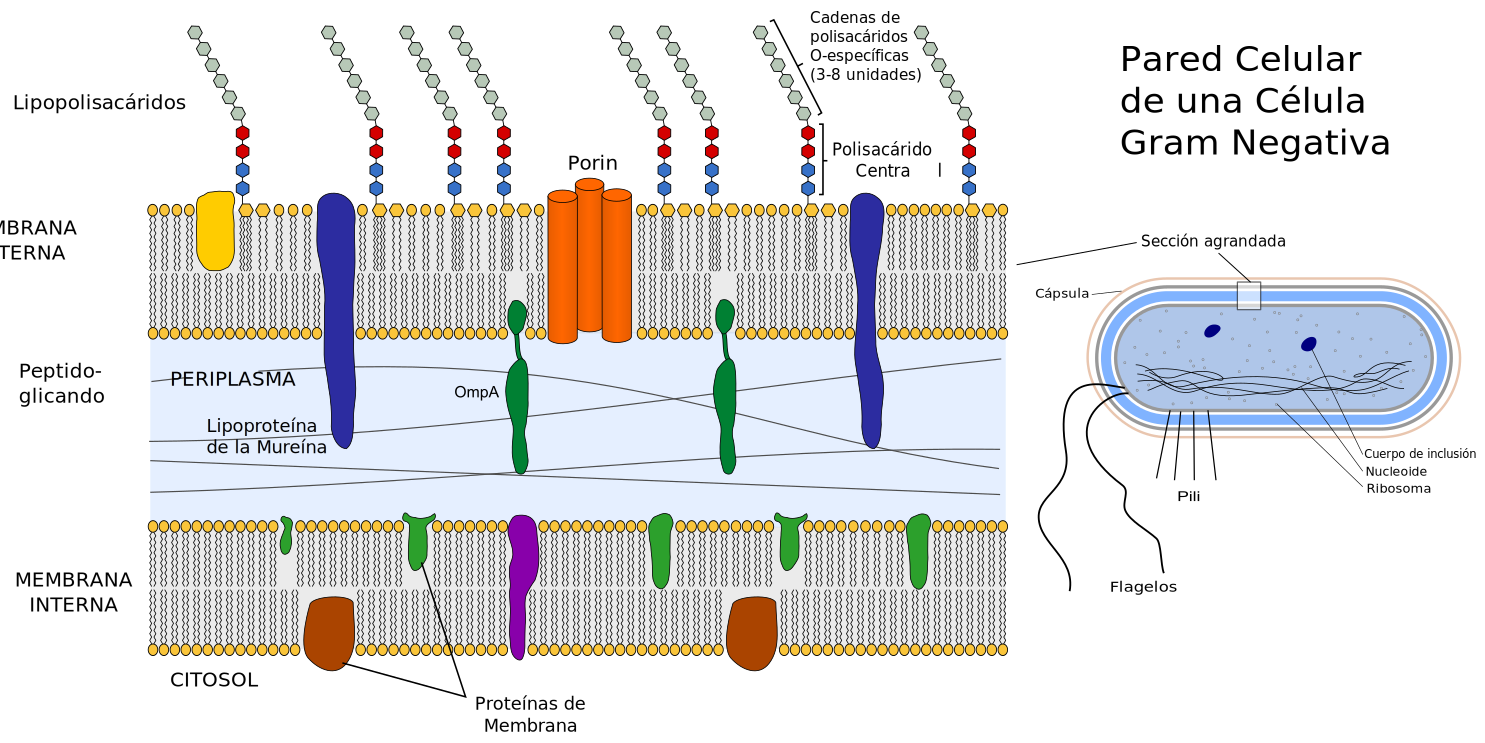
\includegraphics[scale=0.3]{Kap3/cell_wall.pdf}
\caption{Membranas interna y externa de una bacteria gram negativa mostrando algunas de las macromol\'{e}culas que la constituyen. En elmedio de las dos membranas est\'{a} la pared celular que divide el periplasma en dos partes. Traducida de \cite{Dahl2008File:Gram-}}\label{fig:cell}
\end{figure}
Tambi\'{e}n se observan macromol\'{e}culas unidas a cada membrana, algunas de estas son prote\'{i}nas de membrana. Hay prote\'{i}nas de membrana que atraviesan la membrana (prote\'{i}nas integrales de membrana) mientras que otras s\'{o}lamente est\'{a}n ubicadas en el interior o 
el exterior de la c\'{e}lula, estas son conocidas como prote\'{i}nas de membrana perif\'{e}ricas. Incluso, algunas est\'{a}n unidas con grupos no proteicos, tales como carbohidratos y l\'{i}pidos.\\

Para visualizar las membranas se puede usar el microscopio de fuerza at\'{o}mico, que muestra el perfil de la membrana con sus componenentes.\\
\subsection{Transportadores}
La membrana celular al ser hidrof\'{o}bica permite protegerse de la regi\'{o}n extracelular, sin embargo, ella necesita ingresar y expulsar todos los compuestos necesarios para realizar sus procesos metab\'{o}licos. Seg\'{u}n el tama\~{n}o, la concentraci\'{o}n y las cargas relativas de estos compuestos, estos pueden pasar directamente por la membrana lip\'{i}dica, mientras que otras requieren de las prote\'{i}nas de membrana para poder pasar al interior y/o al exterior de la c\'{e}lula. Ah\'{i} entran en juego los \textit{transportadores}, los cuales son prote\'{i}nas integrales de membrana que permiten el ingreso de sustancias al interior y al exterior de las membranas biol\'{o}gicas.\\


Algunas sustancias que pasan directamente por la bicapa fosfolp\'{i}dica son el \ce{O_2} y el \ce{CO_2} que son sustancias peque\~{n}as y apolares, estas pueden pasar por difusi\'{o}n simple, lo cual no requiere un gasto de energ\'{i}a, ya que esto es un efecto dependiente de la organizaci\'{o}n de las moleculas en el espacio, es decir, de los cambios de sus concentraciones en el espacio.\\

Los transportadores se clasifican, de acuerdo al sistema de clasificaci\'{o}n de transportadores \cite{Nelson2011}, en dos categor\'{i}as principales de las cuales se desprenden otras subcategor\'{i}as :
\begin{enumerate}
 \item \textbf{Transportadores}:
 \begin{enumerate}
 \item[1.] Transportadores activos primarios: Son aqu\'{e}llos que requieren un gasto de energ\'{i}a libre para poder mover solutos en contra de su gradiente de concentraci\'{o}n. La forma m\'{a}s conocida para proporcionar energ\'{i}a es mediante la desfosforilaci\'{o}n del ATP.
 \item[2.a] Transportadores activos secundarios (Cotransportadores \cite{Nelson2011}): Son aqu\'{e}llos que est\'{a}n mediados en los que hay un acoplamiento de dos solutos. Mientras uno es transportado a favor del gradiente de concentraci\'{o}n \footnote{Por convenci\'{o}n a favor del gradiente de concentraci\'{o}n significa que pasa de mayor a menor concentraci\'{o}n, es decir, en la direcci\'{o}n contraria al gradiente ``matem\'{a}tico'' $\nabla c$}, proporcionando energ\'{i}a libre, el otro aprovecha esta energ\'{i}a para ir en contra del gradiente de concentraci\'{o}n. Frecuentemente este proceso est\'{a} acompa\~{n}ado de un transporte activo primario, para producir el gradiente favorable de concentraci\'{o}n. Existen dos tipos:
  \begin{enumerate}
 \item[a)] Simportadores: Son los que transportan las dos sustancias en la misma direcci\'{o}n.
 \item[b)] Antiportadores: Son los que transportan las dos sustancias en direcciones contrarias.
 \end{enumerate}
 \item[2.b] Uniportadores: Se da por difusi\'{o}n facilitada, esto es, la prote\'{i}na facilita la difusi\'{o}n a favor del gradiente de concentraci\'{o}n, se presenta debido a que algunas sustancias no son solubles en l\'{i}pidos (iones o sustancias polares) o su tama\~{n}o molecular no les permite pasar.
 \end{enumerate}
 \item  \textbf{Canales i\'{o}nicos}: Los canales se diferencian de los portadores en que no necesitan energ\'{i}a metab\'{o}lica para transportar los iones. Adicional a esto, la raz\'{o}n a la que transportan los iones, es de $10^6$ iones/segundo  (muy alta).
 \end{enumerate}


\section{Simportadores de Sodio Soluto}
Hacia la d\'{e}cada de los a\~{n}os sesenta Robert Crane, ver \cite{Hamilton2013}, estableci\'{o} una relaci\'{o}n acoplada o de \textit{cotransporte} entre el ion de sodio y la glucosa los cuales son absorbidos por el intestino delgado. El conocimiento de este mecanismo ha permitido realizar el tratamiento de la diarrea y del c\'{o}lera mediante la rehidrataci\'{o}n oral. La hip\'{o}tesis del cotransporte ha sido numerosamente validada y ha sido una piedra angular para el entendimiento de el metabolismo de los carbohidratos, claves en la energ\'{e}tica celular. La hip\'{o}tesis del cotransporte tambi\'{e}n se ha extendido a otros organismos vivos, con la diferencia de que el acoplamiento del sodio se puede dar con cualquier otro soluto org\'{a}nico \cite{Faham2008}.\\

Ejemplos de simportadores que transportan el sodio acoplado con otros solutos son el transportador de \ce{Na^{+}/I^{-}} NIS encontrado en las c\'{e}lulas de la gl\'{a}ndula tiroidea, el transportador de  \ce{Na^{+}/Glucosa} SGLT1 encontrado en el intestino delgado (mencionado arriba) y el transportador de  \ce{Na^{+}/Glucosa} SGLT2 encontrado en la nefrona del ri\~{n}on.\\ 

Actualmente los simportadores de \ce{Na^+}-soluto, son una familia de prote\'{i}nas de membrana, denotada como SSS (en ingl\'{e}s Sodium Solute Symporter). La cual pertenece a la superfamilia APC (Por las siglas en ingl\'{e}s Amino acid-poliamine organocation superfamily) de la cual, una familia a resaltar es la NSS, que contiene el cotransportador de leucina y dos \ce{Na^+} LeuT, que posee un plegamiento similar al de los tranportadores mencionados (Com\'{u}nmente conocido como leuT fold o plegamiento de LeuT).\\
\section{Co-transportador vSGLT}\label{sec:esvSGLT}
El cotransportador de Na+/Galactosa presente en la membrana interna de la proteobacteria gram negativa \textit{Vibrio Parahaemolyticus} denotado como vSGLT, es un simportador perteneciente a la familia  SSS \cite{SaierJr.}, es decir, transporta simult\'{a}neamente sodio y galactosa.\\

La caracterizaci\'{o}n molecular del compuesto se realiz\'{o} por primera vez hacia el a\~{n}o 2000 por \cite{Turk2000}, mientras que la determinaci\'{o}n de su estructura fue posible hacia el a\~{n}o 2008 \cite{Faham2008}. Luego, en el a\~{n}o 2010 se determin\'{o} la estructura del mutante K294A (reemplazo de lisina por alanina) en la que aparecen registradas dos $\alpha$ h\'{e}lices adicionales.\\

En la caracterizaci\'{o}n de vSGLT, se encuentra reportada una  masa de 60676 Da y 543 residuos, equivalente a 3854 \'{a}tomos, sin incluir los hidr\'{o}genos. Adem\'{a}s este puede transportar como mon\'{o}mero,  aunque en su forma biol\'{o}gica aparece como d\'{i}mero. Principalmente transporta galactosa, aunque con un menor rendimiento puede transportar glucosa y fructosa, de la misma manera que lo hacen los transportadores SGLT1 Y SGLT2 \cite{SaierJr.}.\\

La estructura tridimensional de vSGLT \cite{Faham2008} se obtiene por difracci\'{o}n de rayos x con un espaciamiento de Bragg entre $2.7\AA$ y $3\AA$ (mejor y peor direcci\'{o}n) y  a una temperatura de $T=100$K. Esta  resoluci\'{o}n es la dada por los rayos x emitidos de una placa de cobre y corresponde al tama\~{n}o al que se alcanzan a percibir los residuos en una prote\'{i}na con posibles errores en los rotameros de las cadenas laterales peque\~{n}as \cite{Huang2007}. Se pasaron por el difract\'{o}metro tres tipos de estructuras cristalinas \ce{P1}, \ce{P2_{1}},  \ce{P2_{1}P2_{1}P2_{1}} que corresponden a los sistemas tricl\'{i}nico, monocl\'{i}nico y ortorr\'{o}mbico \footnote{Existen 7 sistemas cristalinos, cada uno de los cuales cumple una simetr\'{i}a diferente. Cada uno de estos sistemas contiene varios tipos de redes, llamadas redes de Bravais. De acuerdo a la notaci\'{o}n de Germann-Mauguin una celda primitiva se representa con la letra P, ver \cite{VainshteinModernCrystallography}.} respectivamente.\\

En la base de datos del PDB, se encuentra la estructura de vSGLT  como un tetr\'{a}mero con el c\'{o}digo PDB 3DH4, ver figura \ref{fig:3dh4}. La estructura tetram\'{e}rica es la de la celda unitaria. Mientras que en su ensamblaje biol\'{o}gico forma un d\'{i}mero, figura \label{fig:complejo} (a).

\begin{figure}[H]
\centering
\includegraphics[scale=0.1]{Kap3/3dh4tetra.png}
\caption{Tetr\'{a}mero del cotransportador vSGLT (C\'{o}digo pdb 3dh4) como aparece cristalizado.}\label{fig:3dh4}
\end{figure}
La conformaci\'{o}n con la cual se obtuvo la estructura cristalina del simportador fue la conformaci\'{o}n hacia adentro cerrada, es decir, con la galactosa ocluida dentro del simportador tal como se muestra en la figura \ref{fig:3dh4_2}. El sitio del sodio fue determinado de acuerdo a la arquitectura central (core structure) que comparte el simportador con los simportadores que pertenecen a la superfamilia del plegamiento de LeuT, la cual es cercana al sitio Na2 de LeuT. La distancia a la que se encuentran el sodio (ion) y la galactosa (substrato) es $\sim 10 \AA$\\
\begin{figure}[H]
\centering
\includegraphics[scale=0.2]{Kap3/vSGLT_in1.png}
\put(-40,0){(a)}
%\includegraphics[scale=0.07]{Kap3/vSGLT_in2.png}
%\put(-40,0){(b)}
%\vspace{10mm}
\includegraphics[scale=0.25]{Kap3/vSGLT_inward.png}
\put(-50,70){Out}
\put(-50,-5){In}
\put(-60,0){(b)}
\caption{14 segmentos transmembranales de vSGLT con sus $\alpha$ h\'{e}lices representadas por cilindros. La galactosa se muestra  ocluida.(a) Vista desde el periplasma; %(b) vista desde el citoplasma; (c)
(b) vista lateral. Figura tomada de \cite{Faham2008}}\label{fig:3dh4_2}
\end{figure}
El n\'{u}mero de segmentos transmembranales TM es de 14, los cuales est\'{a}n formados por una o a lo sumo dos $\alpha$ h\'{e}lices unidas por lazos. Los segmentos TM est\'{a}n distribuidos entre los residuos \cite{Lomize2012OPMMembranes}:\\

TM1(4-18), TM2(53-77), TM3(82-99), TM4(129-155), TM5(162-177), TM6(188-205), TM7(255-267), TM8(286-305), TM9(348-377), TM10(397-418), TM11(423-443), TM12(458-472), TM13(479-496), TM14(524-545).\\

Debe tenerse en cuenta que el TM2 est\'{a} fragmentado en dos partes:  TM2E(53-64), TM2I(67-77).\\

Posteriormente en \cite{Watanabe2010} aparece una nueva estructura del cotransportador vSGLT mutada en la posici\'{o}n K294A. Esta estructura aparece en su conformaci\'{o}n hacia adentro pero abierta o no ocluida, es decir, con el sustrato liberado. En la base de datos del PDB se encuentra reposada dicha estructura con el c\'{o}digo 2XQ2. Esta estructura difiere de 3DH4 en que all\'{i} se resuelve el segmento TM1, que aunque en la figura \ref{fig:3dh4_2} aparece como una h\'{e}lice, en esta no se conocen las posiciones de los residuos. Adicionalmente, se encuentra una he\'{e}lice adicional al final de la secuencia.\\

En la figura \ref{fig:2xq2} se muestra la unidad asim\'{e}trica (celda unitaria) obtenida por cristalograf\'{i}a de rayos x a una resoluci\'{o}n de $2.73\AA$. La unidad asim\'{e}trica est\'{a} formada por un d\'{i}mero del vSGLT. Cada mon\'{o}mero tiene 15 segmentos transmembranales.\\
\begin{figure}[H]
\centering
\includegraphics[scale=0.2]{Kap3/2xq2.png}
\caption{Unidad asim\'{e}trica del mutante K294A del cotransportador vSGLT mostrando la cadana principal en forma de "cartoon" }\label{fig:2xq2}
\end{figure}
\section{Estudios computacionales del Co-transportador vSGLT}
La estructura del mutante K294A, junto con una nueva caracterizaci\'{o}n bioqu\'{i}mica y simulaciones por din\'{a}mica molecular, todas encontradas en \cite{Watanabe2010} muestran que cuando sale el sodio, la h\'{e}lice 2 (tomada para ellos como 1) se reorienta, permitiendo que se abra la compuerta para que salga posteriormente la galactosa. Al realizar las simulaciones por din\'{a}mica molecular se encuentra que a los $\sim 52$ns la Tyr263 hace su transici\'{o}n entre dos rot\'{a}meros para dejar pasar la galactosa al espacio intracelular,  tal como se muestra en la figura \ref{fig:Y263}.\\
\begin{figure}[ht]
\centering%
\includegraphics[scale=0.4]{Kap3/Y263.png}%
\caption{Abertura de la compuerta Tyr263 para dejar la galactosa en el citoplasma.Tomada de \cite{Watanabe2010}} \label{fig:Y263}
\end{figure}
Posteriormente \cite{Adelman2016}, v\'{i}a simulaciones de din\'{a}mica molecular  encontraron que no existe no existe un orden espec\'{i}fico en que salgan el sodio y la galactosa.
\chapter{Simulaci\'{o}n Computacional}
\section{Modelo de vSGLT con C-$\alpha$}
\begin{figure}
 \centering
  \includegraphics[scale=0.3]{./Kap4/ANM/Ca/BF_plot_100.png}
 \includegraphics[scale=0.3]{./Kap4/ANM/Ca/BF_plot.png}
 \caption{ANM para $R_c=8\AA$ usando a) los primeros 100 modos. b) usando todos los modos}
\end{figure}
\begin{figure}
 \centering
  \includegraphics[scale=0.3]{./Kap4/ANM/Ca/BF_plot_100.png}
 \includegraphics[scale=0.3]{./Kap4/ANM/Ca/BF_plot.png}
 \caption{ANM para $R_c=8\AA$ usando a) los primeros 100 modos. b) usando todos los modos}
\end{figure}
\section{Modelo de vSGLT con C-$\alpha$ y Galactosa}

\section{Mutante K294A de vSGLT con C-$\alpha$}
\chapter{Conclusiones y Recomendaciones}\label{ch:5}
\addcontentsline{toc}{chapter}{\numberline{}Conclusiones y Recomendaciones}
%\section{Conclusiones}
Al realizar el an\'{a}lisis de ANM con un archivo pdb se encontraron los mismos picos en todas las distancias de corte. Para archivo PDB con c\'{o}digo 3DH4 los 5 picos est\'{a}n en los residuos  S209, M318, T343, I386 y W543. Estos lugares correspondieron a sitios que conectan segmentos transmembranales, de ah\'{i} se deben sus altos valores de fluctuaciones ms. Para el archivo PDB con la primera h\'{e}lice resuelta (TM1) se encontraron otros residuos: A47,M318, F542 y G556 que se encontraban poco conectados con los dem\'{a}s residuos.\\

Para archivo PDB con c\'{o}digo 3DH4 al usar las distancias de corte entre $8\AA$ y $9\AA$, se observa que la prote\'{i}na  es menos flexible cuando est\'{a} sin unirse a los sustratos  desde el segmento TM2 hasta el final del segmento TM14. La excepci\'{o}n es el pico presente en el residuo W543 (ver tabla \ref{tab:flu2} del anexo \ref{AnexoB}) que presenta mucha m\'{a}s flexibilidad. Para las otras distancias de corte no ocurre esto.\\

Exceptuando la distancia de corte de $10\AA$, se encontraron cambios en las fluctuaciones ms en los segmentos TM3 y TM7 de la siguiente manera: Dada la flexibilidad del segmento con el cotransportador solo, el cotransportador con el sodio unido tiene m\'{a}s flexibilidad, cuando se unen tanto el sodio como la galactosa el segmento se vuelve menos flexible. Este comportamiento verifica que hay una cooperaci\'{o}n entre el sodio y la galactosa.\\

Las $\alpha$ h\'{e}lices TM1 (primera h\'{e}lice resuelta) y TM15 encontradas en la estructura cristalina de 2XQ2, contribuyen a la estabilidad de la prote\'{i}na cuando se encuentra unida al substrato y al ion, haciendo que los cambios en las fluctuaciones ms sean menores.\\

A diferencia del archivo 3DH4 del ANM previo, usando el PDB con la primera h\'{e}lice resuelta se encontraron cambios en las fluctuaciones ms en el segmento TM2. Este segmento es uno de los que participan almacenando el sodio y la galactosa en el interior del cotransportador.\\

Se encuentra que los residuos y los segmentos transmembranales que generan mayores cambios en los movimientos globales son los reportados previamente en la literatura.\\
%\section{Recomendaciones}
%Se presentan como una serie de aspectos que se podr\'{\i}an realizar en un futuro para emprender investigaciones similares o fortalecer la investigaci\'{o}n realizada. Deben contemplar las perspectivas de la investigaci\'{o}n, las cuales son sugerencias, proyecciones o alternativas que se presentan para modificar, cambiar o incidir sobre una situaci\'{o}n espec\'{\i}fica o una problem\'{a}tica encontrada. Pueden presentarse como un texto con caracter\'{\i}sticas argumentativas, resultado de una reflexi\'{o}n acerca de la tesis o trabajo de investigaci\'{o}n.\\
\begin{appendix}
\chapter{Anexo A: Matriz de Masa del sistema }\label{AnexoA}
En tres dimensiones, como es nuestro caso real, la transformaci\'{o}n \eqref{eq:7} depender\'{a} del modelo escogido. Exceptuando el modelo de redes gaussianas (Gaussian Network Model que por sus siglas en ingl\'{e}s es GNM) la transformaci\'{o}n de coordenadas va de $\mathbf{r}_{i}$ posiciones con $i=1,2,...,N$ ($3N$ coordenadas) a $q_j$ coordenadas $j=1,2,..,3N$:
\begin{equation*}
\mathbf{r}_{i}\longrightarrow q_{j}
\end{equation*}
Con
\begin{equation*}
i=1,2,...,N\mbox{  }j=1,2,..,3N
\end{equation*}
Por cada componente en cartesianas:
\begin{eqnarray}\label{eq:10}
\begin{array}{cccccc}
q_1=x_1-x_{10}&q_4=x_2-x_{20}&\cdots &q_{3i-2}=x_i-x_{i0}&\cdots &q_{3N-2}=x_N-x_{N0} \\
q_2=y_1-y_{10}&q_5=y_2-y_{20}&\cdots &q_{3i-1}=y_i-y_{i0}&\cdots &q_{3N-1}=y_N-y_{N0}\\
q_3=z_1-z_{10}&q_6=z_2-z_{20}&\cdots &q_{3i}=z_i-z_{i0}&\cdots &q_{3N}=z_N-z_{N0}\\
\end{array}
\end{eqnarray}
Para esta transformaci\'{o}n, \eqref{eq:7} se convierte en:
\begin{eqnarray}\label{eq:11}
M_{jk}&=&\sum_{i=1}^{N} m_{i}\left( \delta_{i,3j-2}\delta_{jk}+\delta_{i,3j-1}\delta_{jk}+  \delta_{i,3j}\delta_{jk}\right)\nonumber \\
M_{jk}&=&m_{3j-2}\delta_{jk}+m_{3j-1}\delta_{jk}+m_{3j}\delta_{jk} \nonumber \\
M_{jk}&=&\left( m_{3j-2}+m_{3j-1}+m_{3j} \right) \delta_{jk}
\end{eqnarray}
En \eqref{eq:11} debe resaltarse que para $j=k=3N$, el elemento de matriz $M_{3N,3N}$ requiere las masas $m_{3(3N)-2}=m_{9N-2}$, $m_{3(3N)-1}=m_{9N-1}$ y $m_{3(3N)}=m_{9N}$, sin embargo ! no hay $9N$ masas!, el n\'{u}mero de masas es el mismo n\'{u}mero de nodos: $N$, entonces, para poder calcular la matriz $\mathbf{M}$ es necesario definir lo siguiente:
\begin{equation}\label{eq:12}
m_{N+1},m_{N+2},...,m_{3N}=0
\end{equation}
Como a partir de $N+1$ las masas son nulas, la matriz de masa (que es diagonal) tiene elementos nulos si  
\begin{eqnarray*}
3j-2=N+1\\
j=\frac{N+3}{3} \\
\end{eqnarray*}
Como no siempre $N$ es m\'{u}ltiplo de 3, se escoge el entero menor que este m\'{a}s cerca al valor:
\begin{equation}\label{eq:13}
j=\left \lfloor\frac{N+3}{3}\right \rfloor
\end{equation}
Donde $\lfloor \rfloor$ representa la funci\'{o}n piso.

%\chapter{Anexo:}
\chapter{Anexo B: Fluctuaciones Pico}\label{AnexoB}
En las tablas \ref{tab:flu1} y \ref{tab:flu2} se muestran los identificadores de residuo que presentan m\'{a}ximos o m\'{i}nimos locales (picos) en las figuras \ref{fig:ANM_pre1} \ref{fig:ANM_pre2} y \ref{fig:ANM_pre3}, se muestra por cada distancia de corte entre $7\AA$ y $14\AA$ y para cada modelo de la estructura aplicado (Ca, Ca$+$Na, Ca$+$Na$+$GalCa$+$Gal). Los factores b est\'{a}n normalizados a 1. \\
\begin{table}[ht]
\centering
\begin{adjustbox}{width=1.0\textwidth,center}
 \begin{tabular}[c]{|c|c|}
\multicolumn{2}{c}{$R_c=$8$\AA$}\\\hline
\textbf{Residuo}&\textbf{Factor B}\\\hline
\multicolumn{2}{c}{Con solo C$\alpha$}\\\hline
       253& 0.0416425\\
       251& 0.0415383\\
       249& 0.0377258\\
       479& 0.0376493\\
       250& 0.0373515\\\hline
\multicolumn{2}{c}{C$\alpha$ $+$ Gal}\\\hline
       254& 0.0923907\\
       250& 0.0911848\\
       251& 0.0889088\\
       252& 0.0886782\\
       253& 0.0860388\\\hline
\multicolumn{2}{c}{C$\alpha$ $+$ Gal $+$ Na}\\\hline
       254& 0.0925526\\
       250& 0.0913644\\
       251& 0.0890739\\
       252& 0.0888302\\
       253& 0.0861924\\\hline
\multicolumn{2}{c}{C$\alpha$ $+$ Na}\\\hline
       480&  0.110012\\
        88&  0.109922\\
       479&  0.109521\\
       476&  0.107543\\
       438&  0.106579\\\hline
\end{tabular}
\begin{tabular}[c]{|c|c|}
\multicolumn{2}{c}{$R_c=$9$\AA$}\\\hline
\textbf{Residuo}&\textbf{Factor B}\\\hline
\multicolumn{2}{c}{Con solo C$\alpha$}\\\hline
       253& 0.0416425\\
       251& 0.0415383\\
       249& 0.0377258\\
       479& 0.0376493\\
       250& 0.0373515\\\hline
\multicolumn{2}{c}{C$\alpha$ $+$ Gal}\\\hline
       475&  0.105822\\
       479&  0.105115\\
       250&  0.103229\\
       252&  0.101724\\
        88&  0.100704\\\hline
\multicolumn{2}{c}{C$\alpha$ $+$ Gal $+$ Na}\\\hline
       475&  0.106073\\
       479&  0.105362\\
       250&  0.103468\\
       252&  0.101948\\
        88&  0.100918\\\hline
\multicolumn{2}{c}{C$\alpha$ $+$ Na}\\\hline
       255&  0.116419\\
       257&  0.114597\\
       249&  0.112165\\
       438&  0.112136\\
       258&  0.105612\\\hline
\end{tabular}
\begin{tabular}[c]{|c|c|}
\multicolumn{2}{c}{$R_c=$10$\AA$}\\\hline
\textbf{Residuo}&\textbf{Factor B}\\\hline
\multicolumn{2}{c}{Con solo C$\alpha$}\\\hline
       253&  0.134993\\
       257&  0.133941\\
       258&  0.133659\\
       254&  0.131689\\
       255&  0.130529\\\hline
\multicolumn{2}{c}{C$\alpha$ $+$ Gal}\\\hline
       256&  0.126339\\
       255&  0.125446\\
       257&  0.125102\\
       249&  0.123929\\
       258&  0.117366\\\hline
\multicolumn{2}{c}{C$\alpha$ $+$ Gal $+$ Na}\\\hline
       256&  0.126633\\
       255&  0.125735\\
       257&  0.125394\\
       249&  0.124238\\
       258&   0.11696\\\hline
\multicolumn{2}{c}{C$\alpha$ $+$ Na}\\\hline
       255&  0.134158\\
       257&  0.132059\\
       249&  0.129256\\
       438&  0.129223\\
       258&  0.121705\\\hline
\end{tabular}
\begin{tabular}[c]{|c|c|}
\multicolumn{2}{c}{$R_c=$11$\AA$}\\\hline
\textbf{Residuo}&\textbf{Factor B}\\\hline
\multicolumn{2}{c}{Con solo C$\alpha$}\\\hline
       479& 0.0732422\\
       253& 0.0729239\\
       250& 0.0727664\\
       478&  0.071105\\
       251& 0.0709591\\\hline
\multicolumn{2}{c}{C$\alpha$ $+$ Gal}\\\hline
       250&  0.130337\\
       256&  0.129298\\
       255&  0.129017\\
       258&   0.12784\\
       257&  0.127207\\\hline
\multicolumn{2}{c}{C$\alpha$ $+$ Gal $+$ Na}\\\hline
       259&  0.130679\\
       256&  0.129646\\
       255&  0.128714\\
       258&  0.127578\\
       257&  0.127547\\\hline
\multicolumn{2}{c}{C$\alpha$ $+$ Na}\\\hline
       256&  0.134707\\
       259&  0.134242\\
       255&  0.133804\\
       258&  0.130805\\
       257&  0.130507\\\hline
\end{tabular}
\begin{tabular}[c]{|c|c|}
\multicolumn{2}{c}{$R_c=$12$\AA$}\\\hline
\textbf{Residuo}&\textbf{Factor B}\\\hline
\multicolumn{2}{c}{Con solo C$\alpha$}\\\hline
       479& 0.0643314\\
       253& 0.0640519\\
       250& 0.0639135\\
       478& 0.0624543\\
       251&  0.062326\\\hline
\multicolumn{2}{c}{C$\alpha$ $+$ Gal}\\\hline
       254&  0.115136\\
       253&  0.114893\\
       259&  0.114486\\
       252&  0.111882\\
       256&  0.110051\\\hline
\multicolumn{2}{c}{C$\alpha$ $+$ Gal $+$ Na}\\\hline
       250& 0.0780249\\
       251& 0.0762417\\
       254& 0.0747905\\
       252& 0.0742422\\
       253& 0.0728088\\\hline
\multicolumn{2}{c}{C$\alpha$ $+$ Na}\\\hline
       258&  0.115959\\
       253&  0.113907\\
       255&   0.11262\\
       256&   0.11215\\
       252&  0.111072\\\hline
\end{tabular}
\begin{tabular}[c]{|c|c|}
\multicolumn{2}{c}{$R_c=$13$\AA$}\\\hline
\textbf{Residuo}&\textbf{Factor B}\\\hline
\multicolumn{2}{c}{Con solo C$\alpha$}\\\hline
       478& 0.0980013\\
       252& 0.0977737\\
       250& 0.0951496\\
       480& 0.0945263\\
       479& 0.0905842\\\hline
\multicolumn{2}{c}{C$\alpha$ $+$ Gal}\\\hline
       258&    0.1166\\
       253&  0.114328\\
       255&  0.112683\\
       256&  0.112637\\
       252&  0.111443\\\hline
\multicolumn{2}{c}{C$\alpha$ $+$ Gal $+$ Na}\\\hline
       251& 0.0895345\\
       250& 0.0884175\\
       254& 0.0862215\\
       253& 0.0858509\\
       252& 0.0829043\\\hline
\multicolumn{2}{c}{C$\alpha$ $+$ Na}\\\hline
       256&  0.117632\\
       258&  0.117381\\
       255&  0.117372\\
       252&  0.116511\\
       253&   0.11622\\\hline
\end{tabular}
\begin{tabular}[c]{|c|c|}
\multicolumn{2}{c}{$R_c=$14$\AA$}\\\hline
\textbf{Residuo}&\textbf{Factor B}\\\hline
\multicolumn{2}{c}{Con solo C$\alpha$}\\\hline
       250&   0.10348\\
       476&  0.102362\\
       480&  0.101862\\
       253&  0.101347\\
       479& 0.0985975\\\hline
\multicolumn{2}{c}{C$\alpha$ $+$ Gal}\\\hline
       256&   0.11746\\
       258&   0.11726\\
       255&  0.117135\\
       252&  0.116212\\
       253&   0.11608\\\hline
\multicolumn{2}{c}{C$\alpha$ $+$ Gal $+$ Na}\\\hline
       251& 0.0895255\\
       250& 0.0884151\\
       254& 0.0862144\\
       253& 0.0858443\\
       252& 0.0828968\\\hline
\multicolumn{2}{c}{C$\alpha$ $+$ Na}\\\hline
       256&  0.117624\\
       258&  0.117373\\
       255&  0.117364\\
       252&  0.116503\\
       253&  0.116212\\\hline
\end{tabular}

 \end{adjustbox}
 \caption{Lista de los tres n\'{u}meros de residuo que corresponden a los menores factores B}\label{tab:flu1}
\end{table}
\begin{table}[H]
\centering
\begin{adjustbox}{width=1.0\textwidth,center}
 \begin{tabular}[c]{|c|c|}
\multicolumn{2}{c}{$R_c=$8$\AA$}\\\hline
\textbf{Residuo}&\textbf{Factor B}\\\hline
\multicolumn{2}{c}{Con solo C$\alpha$}\\\hline
       543&  0.999999\\
       318&  0.798209\\
       319&   0.77496\\
       321&  0.741277\\
       317&  0.668767\\
\hline
\multicolumn{2}{c}{C$\alpha$ $+$ Gal}\\\hline
       209&  0.925647\\
       210&  0.879899\\
       318&  0.781582\\
       386&  0.775865\\
       384&  0.773399\\
\hline
\multicolumn{2}{c}{C$\alpha$ $+$ Gal $+$ Na}\\\hline
       209&  0.927167\\
       210&  0.881346\\
       318&  0.782798\\
       386&   0.77716\\
       384&  0.774713\\
\hline
\multicolumn{2}{c}{C$\alpha$ $+$ Na}\\\hline
       209&  0.868804\\
       210&  0.845608\\
       318&  0.827396\\
       211&  0.716527\\
       384&  0.702102\\
\hline
\end{tabular}
\begin{tabular}[c]{|c|c|}
\multicolumn{2}{c}{$R_c=$9$\AA$}\\\hline
\textbf{Residuo}&\textbf{Factor B}\\\hline
\multicolumn{2}{c}{Con solo C$\alpha$}\\\hline
       543&  0.999999\\
       318&  0.798209\\
       319&   0.77496\\
       321&  0.741277\\
       317&  0.668767\\
\hline
\multicolumn{2}{c}{C$\alpha$ $+$ Gal}\\\hline
       209&  0.882793\\
       210&  0.859023\\
       318&   0.84161\\
       211&  0.727772\\
       384&  0.714453\\
\hline
\multicolumn{2}{c}{C$\alpha$ $+$ Gal $+$ Na}\\\hline
       209&  0.884548\\
       210&  0.860736\\
       318&  0.843289\\
       211&  0.729196\\
       384&  0.715938\\
\hline
\multicolumn{2}{c}{C$\alpha$ $+$ Na}\\\hline
       210&  0.851038\\
       385&   0.83699\\
       209&  0.831604\\
       318&  0.789342\\
       211&  0.702455\\
\hline
\end{tabular}
\begin{tabular}[c]{|c|c|}
\multicolumn{2}{c}{$R_c=$10$\AA$}\\\hline
\textbf{Residuo}&\textbf{Factor B}\\\hline
\multicolumn{2}{c}{Con solo C$\alpha$}\\\hline
       209&   0.97897\\
       210&  0.971493\\
       318&  0.781321\\
       311&  0.755165\\
       315&  0.744612\\
\hline
\multicolumn{2}{c}{C$\alpha$ $+$ Gal}\\\hline
       210&  0.997761\\
       385&  0.982432\\
       209&  0.974967\\
       318&  0.926077\\
       211&  0.823312\\
\hline
\multicolumn{2}{c}{C$\alpha$ $+$ Gal $+$ Na}\\\hline
       210&  0.999999\\
       385&  0.984738\\
       209&  0.977157\\
       318&  0.928175\\
       211&  0.825091\\
\hline
\multicolumn{2}{c}{C$\alpha$ $+$ Na}\\\hline
       210&  0.980716\\
       385&  0.964528\\
       209&  0.958321\\
       318&  0.909619\\
       211&  0.809492\\
\hline
\end{tabular}
\begin{tabular}[c]{|c|c|}
\multicolumn{2}{c}{$R_c=$11$\AA$}\\\hline
\textbf{Residuo}&\textbf{Factor B}\\\hline
\multicolumn{2}{c}{Con solo C$\alpha$}\\\hline
       209&  0.857345\\
       386&  0.806943\\
       318&  0.796594\\
       388&  0.790143\\
       384&  0.737336\\
\hline
\multicolumn{2}{c}{C$\alpha$ $+$ Gal}\\\hline
       210&  0.997539\\
       209&  0.923375\\
       318&  0.866003\\
       382&  0.813186\\
       211&  0.803287\\
\hline
\multicolumn{2}{c}{C$\alpha$ $+$ Gal $+$ Na}\\\hline
       210&         1\\
       209&  0.925618\\
       318&  0.868137\\
       382&  0.815369\\
       211&  0.805206\\
\hline
\multicolumn{2}{c}{C$\alpha$ $+$ Na}\\\hline
       210&  0.978538\\
       209&   0.90573\\
       318&  0.848982\\
       382&  0.797229\\
       211&  0.788358\\
\hline
\end{tabular}
\begin{tabular}[c]{|c|c|}
\multicolumn{2}{c}{$R_c=$12$\AA$}\\\hline
\textbf{Residuo}&\textbf{Factor B}\\\hline
\multicolumn{2}{c}{Con solo C$\alpha$}\\\hline
       209&  0.753039\\
       386&  0.708769\\
       318&  0.699679\\
       388&  0.694012\\
       384&   0.64763\\
\hline
\multicolumn{2}{c}{C$\alpha$ $+$ Gal}\\\hline
       210&  0.877561\\
       209&  0.857573\\
       318&  0.737105\\
       211&  0.700336\\
       545&  0.691128\\
\hline
\multicolumn{2}{c}{C$\alpha$ $+$ Gal $+$ Na}\\\hline
       209&  0.999999\\
       318&  0.895038\\
       388&    0.7751\\
       343&  0.764006\\
       210&  0.752476\\
\hline
\multicolumn{2}{c}{C$\alpha$ $+$ Na}\\\hline
       210&   0.94773\\
       209&  0.821616\\
       318&  0.695025\\
       211&  0.676508\\
       545&  0.615122\\
\hline
\end{tabular}
\begin{tabular}[c]{|c|c|}
\multicolumn{2}{c}{$R_c=$13$\AA$}\\\hline
\textbf{Residuo}&\textbf{Factor B}\\\hline
\multicolumn{2}{c}{Con solo C$\alpha$}\\\hline
       209&  0.981844\\
       318&   0.89057\\
       210&  0.832029\\
       317&  0.726279\\
       314&  0.710232\\
\hline
\multicolumn{2}{c}{C$\alpha$ $+$ Gal}\\\hline
       210&  0.978828\\
       209&  0.848552\\
       318&  0.717871\\
       211&  0.698532\\
       545&  0.641043\\
\hline
\multicolumn{2}{c}{C$\alpha$ $+$ Gal $+$ Na}\\\hline
       209&  0.999999\\
       318&  0.907254\\
       210&  0.847078\\
       317&  0.739736\\
       314&  0.723279\\
\hline
\multicolumn{2}{c}{C$\alpha$ $+$ Na}\\\hline
       209&  0.889031\\
       210&  0.874584\\
       318&  0.696198\\
       211&  0.662066\\
       311&  0.656291\\
\hline
\end{tabular}
\begin{tabular}[c]{|c|c|}
\multicolumn{2}{c}{$R_c=$14$\AA$}\\\hline
\textbf{Residuo}&\textbf{Factor B}\\\hline
\multicolumn{2}{c}{Con solo C$\alpha$}\\\hline
       209&  0.947309\\
       210&  0.900641\\
       318&  0.799395\\
       386&  0.792957\\
       384&   0.79044\\
\hline
\multicolumn{2}{c}{C$\alpha$ $+$ Gal}\\\hline
       209&  0.908923\\
       210&  0.894141\\
       318&  0.711833\\
       211&  0.676765\\
       311&  0.670858\\
\hline
\multicolumn{2}{c}{C$\alpha$ $+$ Gal $+$ Na}\\\hline
       209&         1\\
       318&   0.90724\\
       210&   0.84708\\
       317&  0.739725\\
       314&  0.723268\\
\hline
\multicolumn{2}{c}{C$\alpha$ $+$ Na}\\\hline
       209&  0.888968\\
       210&  0.874523\\
       318&  0.696149\\
       211&   0.66202\\
       311&  0.656245\\
\hline
\end{tabular}

 \end{adjustbox}
  \caption{Lista de los tres n\'{u}meros de residuo que corresponden a los mayores factores B}\label{tab:flu2}
\end{table}

\end{appendix}

\addcontentsline{toc}{chapter}{\numberline{}Bibliograf\'{\i}a}
\let\Contentsline\contentsline 
\renewcommand\contentsline[2]{\Contentsline{#1}{}}
%\bibliographystyle{siam}
 \bibliographystyle{plaindin_esp}
%\bibliographystyle{apacite}
\bibliography{Mendeley}
\end{document}